\documentclass[preprint,12pt]{elsarticle}

\usepackage{amsmath}
\usepackage{amssymb}
\usepackage{graphicx}
\usepackage{booktabs}
\usepackage{adjustbox}
\usepackage{hyperref}

% Left empty: the arXiv version is not tied to a journal.
\journal{}

\begin{document}

\begin{frontmatter}
\title{An Exact A Posteriori Error Decomposition for Operator Learning: Conservation, Fluctuation, and the Limit of Branch Capacity}

\author{Xiaochen Yan}


\address{Independent Researcher, Shenzhen, China. ORCID: 0009-0002-9280-4323}
\ead{319914780@qq.com}


\begin{quote}
Repository note: the paragraph below records why the title changed and is not part of the submission. It is stripped from the LaTeX source by \texttt{scripts/md\_to\_tex.py}.
\end{quote}







\begin{abstract}

On periodic Burgers the spatial mean is conserved, so relative L2 can hide that a model predicts nothing beyond a conserved scalar. We decompose squared prediction error exactly into a conserved-mean part and a fluctuation part and prove a hard upper bound on fluctuation skill that depends only on the trunk span.

Against a defined zero-fluctuation reference on 1D Burgers (Nu = 0.001, t = 1.0), MLP DeepONet scores -0.0042 $\pm$ 0.0072 and Fourier DeepONet -0.0934 $\pm$ 0.0886 in per-sample fluctuation $R^2$, while FNO scores +0.6503 $\pm$ 0.0222 on identical data, split and budget.

The deficit is horizon-dependent rather than absolute. Across seven horizons skill decays for every architecture, monotone but for one Fourier reversal, giving an interpolated skill horizon near 0.98 (MLP), 0.86 (Fourier) and 1.94 (FNO). The decay tracks nonlinear spectral evolution, and is absent on linear advection.

An a-priori fluctuation-energy threshold, fitted on two scalar families and never refitted, predicts the sign of skill on held-out settings. The record is stratified since the 55 are not equally informative: 27 of 30 discriminating, 5 of 6 at the boundary, against 16 of 30 for always positive.

Physics-informed training likewise fails, its deficit again localising in the conserved mean, and the dissociation replicates on a second disjoint split. We claim a diagnostic decomposition with two proved propositions and a reproducible negative result, not a theorem for the empirical rule.

\end{abstract}
\begin{keyword}
error decomposition \sep conservation laws \sep spectral bias \sep scientific machine learning \sep reproducibility
\end{keyword}
\end{frontmatter}
\textbf{Preprint --- not peer-reviewed.} This is the version submitted for review; it has not been through peer review and should not be cited as a published result. The code that produced every number in it is archived at \url{https://doi.org/10.5281/zenodo.23765688.} Once a version of record exists, cite that instead of this document.
The study covers six operator families --- linear advection, Burgers at two viscosities, diffusion-sorption, steady 2D Darcy, a three-field compressible system and a two-field reaction-diffusion system --- plus a physics-informed arm. "Family" counts a distinct PDEBench dataset; Burgers at two viscosities and Darcy at two \texttt{beta} values are one family each, giving eight setting-instances in total.
\section{Research question and contribution}

Prior drafts of this study reported a dissociation: better offline basis quality and more stable training fit did not produce better validation error. That statement is descriptive. This version asks what the models actually predict, and answers it with a decomposition that turns the dissociation into a measurement.

\textbf{Claimed contributions} (1-5, 7) are the decomposition, the negative result it measures, and the localisations that follow. Item 6 is an \textbf{empirical regularity found by the study}, reported with its falsification; it is not claimed as a theorem and is not what the decomposition rests on.

\begin{enumerate}
\item A \textbf{mean/fluctuation decomposition}, stated as two propositions with proofs: an exact orthogonal split of squared error into a conserved-mean part and a fluctuation part (Proposition 1), and a hard upper bound on fluctuation skill depending only on the trunk span (Proposition 2). It supplies a defined zero-fluctuation reference and two skill measures that differ in how they weight samples, and it identifies the widely used "input spatial-mean baseline" as a conservation-law predictor.
\item A \textbf{negative result with a boundary rather than a mechanism}: on this protocol DeepONet reproduces a conserved quantity and has no per-sample fluctuation skill, and the skill it does have at short forecast horizons decays to zero as the horizon grows. The decay is quantified as an interpolated \emph{skill horizon} that differs by architecture, and it is shown to track nonlinear spectral evolution rather than elapsed forecast time, because it is absent on linear advection (section 5.6.1).
\item A \textbf{budget control}: the near-zero skill is not undertraining, and additional updates make the per-sample measure worse while leaving total relative L2 flat.
\item A \textbf{measurement warning}: an energy-weighted skill measure can report improvement where the per-sample measure reports degradation. Both are reported throughout.
\item A \textbf{localisation of the binding constraint}. An exact upper bound on fluctuation skill that depends only on the trunk span (section 3.3) shows the reachable set does not shrink with forecast horizon while the map onto it does, so on this protocol the constraint is the branch --- the input-to-coefficient mapping --- and not the trunk basis. This qualifies rather than contradicts the basis-quality line of work in [2].
\item \emph{(Empirical, not claimed as theory.)} A \textbf{prospective predictor, stated with its boundary}. An a-priori fluctuation-energy threshold, fitted on two scalar families and never refitted, predicts the sign of fluctuation skill on held-out settings: 52 of 55 preregistered sign predictions are correct, of which 27 of 30 are on settings that can actually discriminate and 5 of 6 are at the threshold boundary (sections 5.15-5.16). It fails on 1D compressible CFD (3 of 6, every prediction of positive skill wrong) and holds on 2D reaction-diffusion (4 of 4), so the failure is specific to that operator rather than to coupled fields. Both the confirmations and the falsification are reported; nothing was adjusted in response.
\item A \textbf{localisation of where physics-informed training fails}. With no supervision at the target time, the decomposition shows the deficit sits in the conserved mean and not in the fluctuation: the fluctuation share reaches the oracle value while the mean share rises by roughly a factor of four (section 5.11).
\end{enumerate}


The linear-algebra identities below are standard, not new approximation theory. Neither orthonormalization, zero-residual initialization, cosine decay, nor POD truncation is claimed as a new method.

\section{Related work and overlap}

The architectures compared here are DeepONet [10] and the Fourier neural operator [11]. Neither is ours; the contribution is a decomposition applied to both.

\textbf{Relation to a posteriori error estimation.} The decomposition of section 3.1 is an a posteriori error identity in the plain sense that it is evaluated on a trained model's predictions and needs no retraining. It nonetheless differs from the classical finite-element literature [13, 14] in what is bounded, and the difference matters for how section 5 should be read. There the operator is known and the exact solution is not, so the error is unobservable and an \emph{estimator} must be constructed to stand in for it --- the estimator carries the argument. Here the operator is learned but the target is known, so nothing has to be estimated: Proposition 1 is exact by orthogonality, and Proposition 2 bounds what the architecture can represent rather than the error of any particular fit. The two shares are therefore not error estimates but error \emph{accounts}. What they localise is a property of a model class, not a residual of a discretisation to be driven to zero by refinement --- which is why adding updates does not repair it (section 5.10).

Lee and Shin introduce two-step DeepONet training with trunk-first learning followed by branch learning and orthonormalization [1]. Fixed-trunk training and basis orthogonalization are therefore comparison points, not original contributions.

Williams et al. examine learned PI-DeepONet bases, singular-value/coefficient behavior and transfer learning [2]. Our results qualify rather than contradict that line: trunk features matter at short forecast horizons (the Fourier trunk scores +0.4248 against +0.1695 for the MLP trunk at t=0.25) and stop mattering at t=1.00 (-0.0934 against -0.0042). Any claim about trunk basis quality should state the forecast horizon.

Lu et al. compare DeepONet and FNO with practical extensions, including POD-DeepONet, across multiple benchmarks [3]. Their result that architecture choice dominates on these tasks is consistent with ours; our decomposition locates the difference in the fluctuation component rather than in total error. Demo et al. learn a residual correction on a POD basis [8], and Koike et al. study mode selection for sparse networks [9]; a modal-shrinkage line in this repository was closed after failing its predeclared confirmation and is not part of the current argument see UNCERTAINTY\_MODAL\_V1.md.

PDEBench supplies the public data [4]. Zero-initialized residual mechanisms precede this study, for example ReZero [5]; our zero final readout around an input-mean baseline is not identical to ReZero's residual gates and no dynamical-isometry claim is made. Cosine scheduling [6] and large-batch generalization studies [7] are established; we do not present convergence-versus-generalization as a new general discovery, and no sharpness mechanism is claimed. Khodakarami et al. analyse spectral bias in physics-informed and operator learning and report that it is architecture dependent [12], which is consistent with, and independent support for, the horizon-dependent trunk result in section 5.5.

\section{Mean/fluctuation decomposition}

Let \texttt{Y} and \texttt{P} in $R^{m x N}$ be target and predicted fields for \texttt{m} trajectories on the same \texttt{N}-point grid. Write the per-sample spatial mean as \texttt{bar(y)\_j} and the fluctuation as $Y_c = Y - bar(y) 1^T$, and similarly $P_c$.

\subsection{An exact split of squared error}

\textbf{Proposition 1 (orthogonal split).} For any $y_j, p_j \in R^N$, writing $\bar y_j = N^{-1} 1^T y_j$ and $y_{c,j} = y_j - \bar y_j 1$, and likewise for \texttt{p},

\[
  \|p_j - y_j\|^2 = N(\bar p_j - \bar y_j)^2 + \|p_{c,j} - y_{c,j}\|^2 .
\]

Consequently, for any finite collection of samples and any prediction rule,

\[
  \underbrace{\mathbb{E}_j \frac{N(\bar p_j-\bar y_j)^2}{\|y_j\|^2}}_{\text{mean share}}
  +
  \underbrace{\mathbb{E}_j \frac{\|p_{c,j}-y_{c,j}\|^2}{\|y_j\|^2}}_{\text{fluctuation share}}
  = \mathbb{E}_j\,\mathrm{relL2}_j^2 .
\]

\emph{Proof.} Write $p_j - y_j = (\bar p_j - \bar y_j)1 + (p_{c,j} - y_{c,j})$. The two summands are orthogonal because $1^T (p_{c,j} - y_{c,j}) = 0$ by construction, and $\|(\bar p_j - \bar y_j)1\|^2 = N(\bar p_j - \bar y_j)^2$; Pythagoras gives the first identity. Dividing by $\|y_j\|^2$ and averaging over \texttt{j} gives the second. $\blacksquare$

The split is an \textbf{identity}, not an attribution of cause: it holds for every prediction, so it cannot by itself say why a model fails. Its content is that the two shares are exactly additive and separately computable, which is what makes the localisation in section 5 possible.

\texttt{scripts/diagnose\_fluctuation.py} reports both shares and a closure term that the test suite asserts to be zero to machine precision.

\subsection{Two skill measures}

\begin{center}
\begin{adjustbox}{max width=\linewidth}
\small
\begin{tabular}{lll}
\toprule
Measure & Definition & Dominated by \\
\midrule
\texttt{fluctuation\_r2} & $1 - sum_j \|\|p_c-y_c\|\|^2 / sum_j \|\|y_c\|\|^2$ & high-energy samples \\
\texttt{fluctuation\_r2\_per\_sample} & \texttt{1 - (fluctuation share) / (per-sample fluctuation energy)} & every sample equally \\
\bottomrule
\end{tabular}
\end{adjustbox}
\end{center}


Both are referenced to a \textbf{zero-fluctuation} predictor: any prediction whose fluctuation is zero scores 0, including the exact-mean predictor and the all-zero predictor. $R^2$ is therefore invariant to the mean and measures fluctuation skill only; it is never a measure of total accuracy. The manuscript's headline metric is a per-sample mean, so the per-sample measure decides the claims, and the energy-weighted one is reported alongside because the two can disagree in sign (section 5.4).

\subsection{An exact upper bound from the trunk span}

\textbf{Proposition 2 (trunk-span bound).} Let $Phi \in R^{N x p}$ be the trunk feature matrix, let $S = span([Phi, 1])$ and let \texttt{P} be the orthogonal projector onto \texttt{S}. Write $e = E_j \|y_{c,j}\|^2 / \|y_j\|^2$ for the per-sample fluctuation energy. Then every DeepONet output $p_j \in S$ satisfies

\[
  R^2_{\text{per sample}} \;\le\; 1 - \frac{s_{\min}}{e},
  \qquad
  s_{\min} \;=\; \mathbb{E}_j \frac{\|(I-P)\,y_{c,j}\|^2}{\|y_j\|^2} .
\]

Moreover $s_{\min}$ is attained by a per-sample oracle branch, so the bound is tight for the given trunk and cannot be improved without changing \texttt{Phi}.

\emph{Proof.} Since $1 \in S$ and $p_j \in S$, the fluctuation $p_{c,j} = p_j - \bar p_j 1$ also lies in \texttt{S}. Decompose the target fluctuation orthogonally as $y_{c,j} = P y_{c,j} + (I-P) y_{c,j}$. Then

\[
  p_{c,j} - y_{c,j} = \underbrace{(p_{c,j} - P y_{c,j})}_{\in S}
                      - \underbrace{(I-P) y_{c,j}}_{\in S^\perp},
\]

and the two terms are orthogonal, so by Pythagoras $\|p_{c,j} - y_{c,j}\|^2 = \|p_{c,j} - P y_{c,j}\|^2 + \|(I-P)y_{c,j}\|^2 \ge
\|(I-P)y_{c,j}\|^2$. Dividing by $\|y_j\|^2$ and averaging bounds the fluctuation share below by $s_{\min}$, and $R^2_{\text{per sample}} = 1 - (\text{fluctuation share})/e$ gives the claim. For tightness, take $p_j = P y_{c,j} + c\,1 \in S$ for any constant \texttt{c}; its fluctuation is $P y_{c,j}$, which attains equality. Such a $p_j$ is realised by choosing the coefficient vector per sample, i.e. by an oracle branch. $\blacksquare$

The bound is evaluated in section 5.7 on 45 trained trunks and is never violated. This is an identity about the trunk's span, hence a \textbf{hard upper bound}, not an attribution. It requires the trunk but no branch training. Comparing it with achieved skill separates two failure modes: achieved near the bound means the trunk span is binding; achieved far below it means the branch, that is the input-to-coefficient map, is binding. The gap is the amount lost by the branch.

\subsection{The mean baseline is a conservation-law predictor}

For periodic Burgers, \texttt{d/dt int u dx = -[u\^{}2/2] + nu[u\_x] = 0}, so the spatial mean of the target equals that of the input. Measured on the stored data:

\begin{center}
\begin{adjustbox}{max width=\linewidth}
\small
\begin{tabular}{lrrr}
\toprule
Split & corr(mean(x), mean(y)) & mean abs difference & mean abs target mean \\
\midrule
train & 1.000000 & 3.179e-05 & 4.959e-01 \\
validation & 1.000000 & 2.816e-05 & 5.097e-01 \\
test & 1.000000 & 2.977e-05 & 5.012e-01 \\
\bottomrule
\end{tabular}
\end{adjustbox}
\end{center}


Predicting the exact input mean and zero fluctuation therefore yields 0.37577 test mean relative L2, with a fluctuation share of 0.22002 and a mean share of 0. The reported "input spatial-mean baseline" is not a weak strawman: it is the best possible conservation-law predictor, and matching it is a real, nontrivial requirement.

\section{Data, controls and sequential study design}

We use PDEBench's 1D Burgers Nu0.001 file, verified by SHA-256, with 10000 trajectories, 201 stored time layers and 1024 cell-centered spatial points. The primary task maps t=0 to t=1.0 (index 100), with stride-four point sampling to 256 points and no anti-alias filter.

Every input file is pinned to a publisher-checked digest, recorded in each family's \texttt{protocol.json}, and \texttt{src/public\_benchmark.py} refuses to proceed if the file changes:

\begin{center}
\begin{adjustbox}{max width=\linewidth}
\small
\begin{tabular}{llll}
\toprule
File & Source & Identifier & Digest \\
\midrule
\texttt{1D\_Burgers\_Sols\_Nu0.001.hdf5} & HuggingFace \texttt{pdebench/Burgers} & git rev \texttt{97bf5bb5315b} & SHA-256 \texttt{afeeed1c40ce01d2...} \\
\texttt{1D\_Advection\_Sols\_beta0.4.hdf5} & HuggingFace \texttt{pdebench/Advection} & git rev \texttt{33d90a245d98b} & SHA-256 \texttt{d973ff2bb3c2a5ed...} \\
\texttt{1D\_Burgers\_Sols\_Nu0.01.hdf5} & DaRUS \texttt{darus-2986} v8 & datafile 281363 & MD5 \texttt{e6d9a4f62baf9a29...} \\
\texttt{1D\_diff-sorp\_NA\_NA.h5} & DaRUS \texttt{darus-2986} v8 & datafile 133020 & MD5 \texttt{9d466d1213065619...} \\
\texttt{2D\_DarcyFlow\_beta1.0\_Train.hdf5} & DaRUS \texttt{darus-2986} v8 & datafile 133219 & MD5 \texttt{81694ed31306ff2e...} \\
\texttt{2D\_DarcyFlow\_beta0.01\_Train.hdf5} & DaRUS \texttt{darus-2986} v8 & datafile 133217 & MD5 \texttt{d05c287d4c0b7d31...} \\
\texttt{2D\_DarcyFlow\_beta10.0\_Train.hdf5} & DaRUS \texttt{darus-2986} v8 & datafile 133220 & MD5 \texttt{a7f23cf8011fc211...} \\
\texttt{1D\_CFD\_Rand\_Eta0.01\_Zeta0.01\_periodic\_Train.hdf5} & DaRUS \texttt{darus-2986} v8 & datafile 164672 & MD5 \texttt{2fdd00138f1d7abc...} \\
\texttt{2D\_diff-react\_NA\_NA.h5} & DaRUS \texttt{darus-2986} v8 & datafile 133017 & MD5 \texttt{b8d0b86064193195...} \\
\bottomrule
\end{tabular}
\end{adjustbox}
\end{center}


The Burgers SHA-256 was re-verified against the local file on 2026-10-08 and matches exactly. Digests are truncated here for layout; full values are in \texttt{protocol.json} and in \texttt{scripts/download\_darus.py} and \texttt{scripts/download\_pdebench.py}. The generator uses epsilon/pi as the diffusion coefficient.

The initial split is 1000 training, 200 validation and 200 test trajectories, sampled with split seed 20260922. Input/target scalar normalization uses training arrays only. DeepONet uses 64 trunk features and three-layer, width-128 branch/trunk MLPs; the alternative trunk uses fixed random Fourier input features. The FNO reference has four blocks, width 32 and 16 spectral modes. All training seeds are 0-4.

\begin{center}
\begin{adjustbox}{max width=\linewidth}
\small
\begin{tabular}{lrll}
\toprule
Family & Run records & Main intervention & Evaluation status \\
\midrule
public\_fixed\_t1\_v1 & 15 & MLP/Fourier DeepONet and FNO, 1500 updates & Train/validation/test; exploratory subset \\
public\_coefficients\_v1 & 40 & Conditioning x mean offset, 3000 branch updates & Same exploratory split \\
public\_smallfit\_v1 & 60 & n=32/128/1000 x random/zero readout & Train/validation only \\
public\_stability\_v1 & 40 & Constant/cosine LR x batch 32/128, n=128 & Train/validation only \\
public\_steps5k\_v1 & 15 & Same three architectures, 5000 updates & Train/validation/test \\
public\_steps20k\_v1 & 15 & Same three architectures, 20000 updates & Train/validation/test \\
public\_horizon\_t010\_v1 & 15 & Target time 0.10, 1500 updates & Train/validation/test \\
public\_horizon\_t025\_v1 & 15 & Target time 0.25, 1500 updates & Train/validation/test \\
public\_horizon\_t050\_v1 & 15 & Target time 0.50, 1500 updates & Train/validation/test \\
public\_horizon\_t075\_v1 & 15 & Target time 0.75, 1500 updates & Train/validation/test \\
public\_horizon\_t150\_v1 & 15 & Target time 1.50, 1500 updates & Train/validation/test \\
public\_horizon\_t200\_v1 & 15 & Target time 2.00, 1500 updates & Train/validation/test \\
public\_wcmatch3500\_v1 & 10 & DeepONet only, 3500 updates (wall-clock matched to FNO at 1500) & Train/validation/test \\
diffsorp\_in020\_t*\_v1 & 90 & Diffusion-sorption, input layer 20, six targets t=125..500 & Train/validation/test \\
\bottomrule
\end{tabular}
\end{adjustbox}
\end{center}


The diffusion-sorption input is layer 20 rather than layer 0 because the stored initial state is spatially constant for every sample; see section 5.6.2 and THIRD\_PDE\_DIFFSORP\_V1.md. Its protocol and prediction were committed before any run on that data.

Horizon variants are prepared by calling \texttt{src.public\_benchmark.prepare} with \texttt{time\_index} 25 and 50 and the \textbf{same split seed and sizes}, so the trajectories are identical and only the target time changes. This is a sensitivity check over forecast horizon, \textbf{not a second PDE}.

These families were designed sequentially after inspecting preceding results. Protocols were fixed before their respective launches, not preregistered as one independent confirmatory study. Ten stability controls reproduce earlier results exactly and are not independent replicates. The test split was exposed during early exploratory development.

Every number in sections 5.1-5.5 was recomputed from stored checkpoints by \texttt{scripts/diagnose\_fluctuation.py}, which compares each recomputed \texttt{mean\_relative\_l2} against the value stored in that run's \texttt{result.json}. All recomputations reproduce their stored metrics exactly ($max_abs_metric_difference = 0.00e+00$ in every family), so the decomposition is applied to a faithful reconstruction rather than an approximation.

\section{Results}

\subsection{Representability is not operator accuracy}

\begin{center}
\begin{adjustbox}{max width=\linewidth}
\small
\begin{tabular}{lr}
\toprule
Initial method & Test mean relative L2 (mean $\pm$ seed SD) \\
\midrule
Input spatial-mean baseline & 0.37577 \\
MLP DeepONet & 0.39357 $\pm$ 0.01014 \\
Fourier DeepONet & 0.41231 $\pm$ 0.01344 \\
FNO & 0.22835 $\pm$ 0.00680 \\
\bottomrule
\end{tabular}
\end{adjustbox}
\end{center}


Both initial DeepONets fail to beat the conservation-law baseline while FNO beats it by a wide margin. Equal update counts do not match parameter counts or compute (section 5.9).

\subsection{Fluctuation skill at t = 1.0}

\begin{center}
\begin{adjustbox}{max width=\linewidth}
\small
\begin{tabular}{lrrrrr}
\toprule
Method & Test relL2 & $R^2$ (energy) & \textbf{$R^2$ (per sample)} & mean share & fluctuation share \\
\midrule
oracle input mean & 0.37577 & 0.0000 & \textbf{0.0000} & 0.0000 & 0.2200 \\
MLP DeepONet & 0.39357 & -0.0056 $\pm$ 0.0094 & \textbf{-0.0042 $\pm$ 0.0072} & 0.0180 & 0.2209 \\
Fourier DeepONet & 0.41231 & -0.0124 $\pm$ 0.0356 & \textbf{-0.0934 $\pm$ 0.0886} & 0.0340 & 0.2406 \\
FNO & 0.22835 & +0.6282 $\pm$ 0.0187 & \textbf{+0.6503 $\pm$ 0.0222} & 0.0023 & 0.0769 \\
\bottomrule
\end{tabular}
\end{adjustbox}
\end{center}


MLP DeepONet's fluctuation share (0.2209) is indistinguishable from the zero-fluctuation reference (0.2200): at 1500 updates it predicts the fluctuation no better than not predicting it at all, and its remaining error over the oracle comes from the mean component. FNO reduces the fluctuation share by 65\% and its mean share by a further order of magnitude.

\subsection{No intervention produces positive fluctuation skill}

\texttt{scripts/diagnose\_fluctuation.py} recomputed all 175 stored runs of the original four families plus the 5k and 20k families. Per-sample fluctuation $R^2$ by family (mean $\pm$ SD over the runs in that family):

\begin{center}
\begin{adjustbox}{max width=\linewidth}
\small
\begin{tabular}{llrr}
\toprule
Family & Split & MLP DeepONet & Fourier DeepONet \\
\midrule
public\_fixed\_t1\_v1 (1500) & test & -0.0042 $\pm$ 0.0072 & -0.0934 $\pm$ 0.0886 \\
public\_coefficients\_v1 (3000) & test & -0.1286 $\pm$ 0.1054 & -0.3030 $\pm$ 0.1558 \\
public\_stability\_v1 (3000) & validation & -0.6438 $\pm$ 0.2273 & -1.4062 $\pm$ 0.1736 \\
public\_scale1000\_v1 (3000) & validation & -0.0354 $\pm$ 0.0556 & -0.3181 $\pm$ 0.0895 \\
public\_smallfit\_v1 (3000) & validation & -2.2911 $\pm$ 4.0722 & -5.5548 $\pm$ 8.7244 \\
\bottomrule
\end{tabular}
\end{adjustbox}
\end{center}


Not one configuration, across trunk architecture, whitening, mean lifting, zero initialization, schedule, batch size and training-subset size, scores above the zero-fluctuation reference. Interventions that improve fitting score worse than the end-to-end baselines, which is the dissociation reported in earlier drafts, now measured on the component that causes it.

\subsection{More updates do not help, and hurt the per-sample measure}

\begin{center}
\begin{adjustbox}{max width=\linewidth}
\small
\begin{tabular}{llrrr}
\toprule
Budget & Method & Test relL2 & $R^2$ (energy) & \textbf{$R^2$ (per sample)} \\
\midrule
1500 & MLP DeepONet & 0.39357 & -0.0056 $\pm$ 0.0094 & \textbf{-0.0042 $\pm$ 0.0072} \\
1500 & Fourier DeepONet & 0.41231 & -0.0124 $\pm$ 0.0356 & \textbf{-0.0934 $\pm$ 0.0886} \\
1500 & FNO & 0.22835 & +0.6282 $\pm$ 0.0187 & \textbf{+0.6503 $\pm$ 0.0222} \\
5000 & MLP DeepONet & 0.39729 & +0.0165 $\pm$ 0.0159 & \textbf{-0.0640 $\pm$ 0.0503} \\
5000 & Fourier DeepONet & 0.40250 & +0.0175 $\pm$ 0.0450 & \textbf{-0.1272 $\pm$ 0.0787} \\
5000 & FNO & 0.21619 & +0.5864 $\pm$ 0.0166 & \textbf{+0.6830 $\pm$ 0.0325} \\
20000 & MLP DeepONet & 0.39311 & +0.2126 $\pm$ 0.0557 & \textbf{-0.2470 $\pm$ 0.1304} \\
20000 & Fourier DeepONet & 0.47689 & -0.1623 $\pm$ 0.0609 & \textbf{-0.8037 $\pm$ 0.2393} \\
20000 & FNO & 0.22243 & +0.5538 $\pm$ 0.0139 & \textbf{+0.6660 $\pm$ 0.0170} \\
50000 & MLP DeepONet & 0.42075 & +0.1496 $\pm$ 0.0484 & \textbf{-0.4157 $\pm$ 0.1901} \\
50000 & Fourier DeepONet & 0.51959 & -0.2974 $\pm$ 0.0631 & \textbf{-1.1099 $\pm$ 0.2875} \\
50000 & FNO & 0.22190 & +0.5661 $\pm$ 0.0131 & \textbf{+0.6659 $\pm$ 0.0148} \\
\bottomrule
\end{tabular}
\end{adjustbox}
\end{center}


Two readings, and the second is the one that matters:

\begin{enumerate}
\item \textbf{Undertraining is not the explanation.} Across a 33x budget range the total relative L2 of MLP DeepONet never improves (0.39357 / 0.39729 / 0.39311 / 0.42075) and FNO is stable (0.22835 / 0.21619 / 0.22243 / 0.22190). The ranking never changes, and at the largest budget DeepONet is worse, not better.
\item \textbf{The energy-weighted measure would have produced a false positive.} At 20000 updates MLP DeepONet reads +0.2126 energy-weighted but -0.2470 per sample: improvement is concentrated in high-energy samples while typical samples get worse. Since the manuscript's metric is a per-sample mean, the per-sample measure decides the claim and the energy-weighted one is reported only alongside it.
\end{enumerate}


The normalized mean error also grows with budget for MLP DeepONet (0.081 -> 0.076 -> 0.111 -> 0.138) while staying at 0.024-0.034 for FNO, so extra updates trade conserved-mean accuracy for fluctuation fitting with no net gain.

\subsection{A skill horizon: the deficit is horizon-dependent and shared}

Same 1500-update budget, same trajectories and split, only the target time changes. Seven horizons are run to trace the decay rather than assert a trend from three points.

\begin{center}
\begin{adjustbox}{max width=\linewidth}
\small
\begin{tabular}{rrrrr}
\toprule
t & fluctuation energy & MLP DeepONet & Fourier DeepONet & FNO \\
\midrule
0.10 & 0.5939 & +0.2199 $\pm$ 0.0554 & +0.6390 $\pm$ 0.0142 & +0.9859 $\pm$ 0.0047 \\
0.25 & 0.4785 & +0.1695 $\pm$ 0.0154 & +0.4248 $\pm$ 0.0168 & +0.9474 $\pm$ 0.0058 \\
0.50 & 0.3580 & +0.1238 $\pm$ 0.0137 & +0.2510 $\pm$ 0.0389 & +0.8369 $\pm$ 0.0075 \\
0.75 & 0.2841 & +0.0539 $\pm$ 0.0023 & +0.0675 $\pm$ 0.0701 & +0.7378 $\pm$ 0.0089 \\
1.00 & 0.2367 & -0.0042 $\pm$ 0.0072 & -0.0934 $\pm$ 0.0886 & +0.6503 $\pm$ 0.0222 \\
1.50 & 0.1786 & -0.0813 $\pm$ 0.0261 & -0.4064 $\pm$ 0.1757 & +0.4051 $\pm$ 0.0217 \\
2.00 & 0.1428 & -0.0918 $\pm$ 0.0491 & -0.3774 $\pm$ 0.0571 & -0.0586 $\pm$ 0.2357 \\
\bottomrule
\end{tabular}
\end{adjustbox}
\end{center}


(per-sample $R^2$ on the test split.)

\textbf{All three architectures lose their fluctuation skill as the horizon grows, and FNO loses it too at t = 2.00.} The deficit is therefore a property of the task's difficulty first and of the architecture second: what differs is \emph{where} each architecture crosses zero. Interpolating linearly between the bracketing horizons gives a \textbf{skill horizon} at which per-sample fluctuation $R^2$ reaches zero:

\begin{center}
\begin{adjustbox}{max width=\linewidth}
\small
\begin{tabular}{llr}
\toprule
Model & bracketing horizons & \textbf{skill horizon (interpolated)} \\
\midrule
Fourier DeepONet & 0.75 (+0.0675) to 1.00 (-0.0934) & \textbf{\textasciitilde{}0.86} \\
MLP DeepONet & 0.75 (+0.0539) to 1.00 (-0.0042) & \textbf{\textasciitilde{}0.98} \\
FNO & 1.50 (+0.4051) to 2.00 (-0.0586) & \textbf{\textasciitilde{}1.94} \\
\bottomrule
\end{tabular}
\end{adjustbox}
\end{center}


FNO's skill horizon is about 2.0x that of MLP DeepONet and 2.3x that of the Fourier-trunk variant. Note that the Fourier trunk is the better trunk at short horizons (+0.6390 against +0.2199 at t = 0.10) and the worse one at long horizons (-0.3774 against -0.0918 at t = 2.00), so trunk-feature claims must state the horizon; this qualifies, rather than contradicts, the basis-quality line of work in [2].

The fluctuation energy fraction decreases monotonically over the same horizons (0.5939 -> 0.1428) and can be computed from the data before any training, so it is an a-priori monotone proxy for horizon difficulty. It does \textbf{not} by itself predict skill across architectures: at a fixed fluctuation energy the three models differ by up to 0.8 in $R^2$. Skill decreases with horizon in every architecture, but only MLP DeepONet and FNO do so monotonically: the Fourier trunk reverses once, from -0.4064 +- 0.1757 at $t = 1.50$ to -0.3774 +- 0.0571 at $t = 2.00$. That single reversal is why the within-Burgers rank correlation between fluctuation energy and skill is 0.964 for the Fourier trunk where it is 1.000 for the other two. The curve itself is set by the architecture.

\subsection{Other operators and a viscosity ladder}

Two controls were run at the same 1500-update budget, seeds, architectures and split. Both use \texttt{scripts/prepare\_*\_horizons.py}, which reuse the extraction and splitting helpers unchanged rather than editing \texttt{prepare()}, because that function pins the Burgers digest and would change \texttt{source\_hash()} in every run identity. The layouts are identical, so training and diagnostics run unmodified, and all recomputations reproduce stored metrics exactly.

\subsubsection{Linear advection}

The Burgers result could be a generic consequence of forecasting further into the future rather than a consequence of nonlinear evolution. To separate these, the same seven horizons, budget, seeds and architectures were run on PDEBench 1D \textbf{linear advection} (beta = 0.4, periodic), whose solution is a pure translation of the initial field.

\begin{center}
\begin{adjustbox}{max width=\linewidth}
\small
\begin{tabular}{rrrrr}
\toprule
t & fluctuation energy & MLP DeepONet & Fourier DeepONet & FNO \\
\midrule
0.10 & 0.6446 & +0.2531 $\pm$ 0.0900 & +0.9228 $\pm$ 0.0354 & +0.9994 $\pm$ 0.0000 \\
0.25 & 0.6446 & +0.2427 $\pm$ 0.0318 & +0.9415 $\pm$ 0.0171 & +0.9994 $\pm$ 0.0001 \\
0.50 & 0.6446 & +0.2058 $\pm$ 0.0616 & +0.9466 $\pm$ 0.0147 & +0.9994 $\pm$ 0.0000 \\
0.75 & 0.6446 & +0.2295 $\pm$ 0.0423 & +0.9278 $\pm$ 0.0310 & +0.9994 $\pm$ 0.0000 \\
1.00 & 0.6446 & +0.1817 $\pm$ 0.0092 & +0.9424 $\pm$ 0.0180 & +0.9994 $\pm$ 0.0000 \\
1.50 & 0.6446 & +0.2390 $\pm$ 0.0309 & +0.9456 $\pm$ 0.0134 & +0.9994 $\pm$ 0.0000 \\
2.00 & 0.6446 & +0.2047 $\pm$ 0.0031 & +0.9354 $\pm$ 0.0178 & +0.9994 $\pm$ 0.0000 \\
\bottomrule
\end{tabular}
\end{adjustbox}
\end{center}


Two things change at once, and both matter:

\begin{enumerate}
\item \textbf{Fluctuation energy is constant across horizons} (0.6446 at every t), as it must be for pure translation, against a monotone decay from 0.5939 to 0.1428 on Burgers.
\item \textbf{No architecture shows a skill horizon.} MLP DeepONet stays within +0.18 to +0.25, Fourier DeepONet within +0.92 to +0.95 and FNO at +0.9994, with no trend in t. The ranges are the observed extrema over the seven horizons, not confidence intervals; five seeds share one split (section 6).
\end{enumerate}


So the decay measured on Burgers is not a generic effect of forecasting further ahead. It appears in the problem whose fluctuation spectrum evolves nonlinearly and is absent in the problem where the fluctuation is merely transported. This is the control that makes the skill horizon interpretable rather than descriptive.

It also sharpens the trunk-feature question. On advection the Fourier trunk is dramatically better than the MLP trunk (+0.94 against +0.21), consistent with translation being a phase shift in a Fourier basis; on Burgers that advantage is present at t=0.10 (+0.6390 against +0.2199) and reverses by t=2.00 (-0.3774 against -0.0918). A trunk that is well matched to the \emph{linear} part of the operator is not automatically well matched once nonlinear steepening dominates.

\subsubsection{A third class: diffusion-dominated, dissipative}

PDEBench 1D diffusion-sorption (\texttt{t} in [0, 500], 101 layers) is parabolic and dissipative with no shocks and no translation. \textbf{Its stored $t = 0$ state is spatially constant for every sample} (spatial standard deviation below 4e-8; only the constant value varies), so it carries one degree of freedom and would make the task "generate a field from a scalar". The input is therefore layer 20 ($t = 100$, spatial standard deviation 0.2390) and all six targets are strictly later. This caveat is recorded in every protocol file; it was found by checking the data, and an earlier preparation bug that silently made one horizon an identity map was caught by the same check.

\begin{center}
\begin{adjustbox}{max width=\linewidth}
\small
\begin{tabular}{rrrrr}
\toprule
t & fluctuation energy & MLP DeepONet & Fourier DeepONet & FNO \\
\midrule
125 & 0.7333 & +0.9983 $\pm$ 0.0014 & +0.9998 $\pm$ 0.0003 & +1.0000 $\pm$ 0.0000 \\
200 & 0.7173 & +0.9990 $\pm$ 0.0010 & +1.0000 $\pm$ 0.0000 & +1.0000 $\pm$ 0.0000 \\
275 & 0.7004 & +0.9988 $\pm$ 0.0012 & +1.0000 $\pm$ 0.0000 & +1.0000 $\pm$ 0.0000 \\
350 & 0.6834 & +0.9997 $\pm$ 0.0002 & +0.9999 $\pm$ 0.0001 & +1.0000 $\pm$ 0.0000 \\
425 & 0.6667 & +0.9998 $\pm$ 0.0001 & +0.9999 $\pm$ 0.0001 & +1.0000 $\pm$ 0.0000 \\
500 & 0.6506 & +0.9999 $\pm$ 0.0001 & +0.9999 $\pm$ 0.0001 & +1.0000 $\pm$ 0.0000 \\
\bottomrule
\end{tabular}
\end{adjustbox}
\end{center}


No architecture shows any skill decay. The fluctuation energy \emph{does} decay here (0.7333 to 0.6506), just as it does on Burgers, yet no zero crossing occurs, because the energy never approaches any architecture's threshold. That asymmetry is the strongest evidence for the threshold form of the rule in section 5.8 as opposed to "a longer forecast is harder".

\textbf{Stated weakness:} 99\% of the target fluctuation energy lies in a single spatial mode at every horizon, so all three models score essentially 1.000 and the setting does not discriminate between architectures. A confirmation here is weak support; a falsification would have been strong evidence. No setting on this PDE lies near a threshold, so the rule's boundary remains untested out of sample.

\subsubsection{A viscosity ladder: the rule at its boundary}

Section 5.6.2 confirms the rule where every model saturates, which is easy. A stronger test needs settings that straddle a threshold. Burgers at $Nu = 0.01$, ten times the viscosity, dissipates faster, so the fluctuation energy crosses the thresholds earlier. Its protocol and all 21 sign predictions were committed before any run on that data (VISCOSITY\_NU001\_V1.md); the thresholds are those fitted on Nu0.001 plus advection and were not refitted.

\begin{center}
\begin{adjustbox}{max width=\linewidth}
\small
\begin{tabular}{rrrrrl}
\toprule
t & fluctuation energy & MLP DeepONet & Fourier DeepONet & FNO & predicted \\
\midrule
0.10 & 0.5661 & +0.2346 $\pm$ 0.0521 & +0.6891 $\pm$ 0.0215 & +0.9975 $\pm$ 0.0004 & + / + / + \\
0.25 & 0.4507 & +0.1737 $\pm$ 0.0126 & +0.4392 $\pm$ 0.0336 & +0.9800 $\pm$ 0.0038 & + / + / + \\
0.50 & 0.3320 & +0.1500 $\pm$ 0.0152 & +0.1878 $\pm$ 0.0747 & +0.9519 $\pm$ 0.0060 & + / + / + \\
0.75 & 0.2596 & +0.0628 $\pm$ 0.0215 & -0.0122 $\pm$ 0.0795 & +0.8751 $\pm$ 0.0126 & + / - / + \\
1.00 & 0.2131 & -0.0273 $\pm$ 0.0159 & -0.2443 $\pm$ 0.1387 & +0.8072 $\pm$ 0.0335 & - / - / + \\
1.50 & 0.1559 & -0.2387 $\pm$ 0.0258 & -0.8703 $\pm$ 0.4734 & +0.4670 $\pm$ 0.0419 & - / - / + \\
2.00 & 0.1217 & -0.2972 $\pm$ 0.1299 & -1.1128 $\pm$ 0.3465 & -0.2219 $\pm$ 0.4127 & - / - / - \\
\bottomrule
\end{tabular}
\end{adjustbox}
\end{center}


\textbf{All 21 predictions are correct} (7/7 per architecture), including every crossing. The interpolated skill horizons are:

\begin{center}
\begin{adjustbox}{max width=\linewidth}
\small
\begin{tabular}{lrrrr}
\toprule
Model & predicted from the rule & measured here & measured at Nu=0.001 & absolute error \\
\midrule
Fourier DeepONet & 0.740 & \textbf{0.735} & 0.860 & 0.005 \\
MLP DeepONet & 0.860 & \textbf{0.924} & 0.980 & 0.064 \\
FNO & 1.650 & \textbf{1.839} & 1.940 & 0.189 \\
\bottomrule
\end{tabular}
\end{adjustbox}
\end{center}


All three are shorter than at Nu=0.001, as predicted. The error grows with horizon length, which is what linear interpolation over a coarse grid implies at the far end of the ladder. This is a parameter ladder on one operator, so it shows the rule tracks a physical parameter; it does not by itself show the rule transfers to a new operator class.

\subsubsection{A steady elliptic operator, and what it says about the mean baseline}

PDEBench 2D Darcy is steady, elliptic and two-dimensional: \texttt{nu (10000,128,128)} is a coefficient field and \texttt{tensor (10000,1,128,128)} the solution, subsampled with stride 2 to 64x64. It differs from every other family in three independent ways, and its protocol and prediction were committed before any run (DARCY\_ELLIPTIC\_V1.md). Two new files supply the 2D machinery (\texttt{src/fno2d.py}, \texttt{scripts/run\_darcy\_benchmark.py}); \texttt{src/fno.py} was not edited because it is hashed into every existing run identity.

\begin{center}
\begin{adjustbox}{max width=\linewidth}
\small
\begin{tabular}{lrrr}
\toprule
Model & test relL2 & \textbf{$R^2$ per sample} & $R^2$ energy-weighted \\
\midrule
MLP DeepONet & 0.26353 & +0.7614 $\pm$ 0.0160 & +0.8081 \\
Fourier DeepONet & 0.16450 & +0.9153 $\pm$ 0.0079 & +0.9333 \\
FNO & 0.08330 & +0.9790 $\pm$ 0.0009 & +0.9731 \\
\bottomrule
\end{tabular}
\end{adjustbox}
\end{center}


The a-priori fluctuation energy is 0.4964, above every threshold, so positive skill was predicted for all three: \textbf{3 of 3 correct}. The rule therefore transfers from 1D evolution problems to a steady elliptic operator with the thresholds unchanged.

\textbf{This family also settles what the mean baseline means.} The input-output mean correlation is \textbf{-0.873}, so no conservation law links them, and the input-spatial-mean predictor gives a test relative L2 of \textbf{3.6843} --- far worse than useless. On Burgers the identical construction was a genuine conservation-law predictor at 0.37577. The comparison shows that the standing of the mean baseline is a property of the operator's physics, not of the metric or of the architecture. The zero-fluctuation reference, by contrast, needs no physics: it is well defined for any field, which is why the skill measure carries over unchanged.

\subsection{The binding constraint is the branch, not the trunk}

Section 3.3 gives an exact upper bound on fluctuation skill that depends only on the trunk span. \texttt{scripts/skill\_bound.py} evaluates it on the trained trunks of nine settings, using the same rcond as the projection audit.

\begin{center}
\begin{adjustbox}{max width=\linewidth}
\small
\begin{tabular}{llrrrr}
\toprule
Setting & Trunk & basis rank & \textbf{bound} & achieved & \textbf{branch gap} \\
\midrule
Advection t = 1.00 & Fourier & 62.8 & +1.0000 $\pm$ 0.0000 & +0.9424 & \textbf{0.058} \\
Advection t = 2.00 & Fourier & 62.2 & +0.9999 $\pm$ 0.0000 & +0.9354 & \textbf{0.065} \\
Burgers t = 0.25 & Fourier & 42.6 & +0.9590 $\pm$ 0.0044 & +0.4248 & 0.534 \\
Burgers t = 1.00 & Fourier & 39.4 & +0.9737 $\pm$ 0.0062 & -0.0934 & 1.067 \\
Burgers t = 2.00 & Fourier & 39.6 & +0.9845 $\pm$ 0.0045 & -0.3774 & 1.362 \\
Advection t = 1.00 & MLP & 7.4 & +0.5785 $\pm$ 0.0458 & +0.1817 & 0.397 \\
Burgers t = 0.25 & MLP & 6.8 & +0.5855 $\pm$ 0.0459 & +0.1695 & 0.416 \\
Burgers t = 1.00 & MLP & 4.4 & +0.5072 $\pm$ 0.0516 & -0.0042 & 0.511 \\
Burgers t = 2.00 & MLP & 4.2 & +0.5180 $\pm$ 0.0462 & -0.0918 & 0.610 \\
\bottomrule
\end{tabular}
\end{adjustbox}
\end{center}


The bound is never violated in any of the 45 evaluated trunks, which is the empirical check that the statement in section 3.3 holds on real checkpoints and not only on paper.

Three consequences:

\begin{enumerate}
\item \textbf{The Fourier trunk's span is not the constraint anywhere.} Its bound is 0.96 to 1.00 on \emph{both} PDEs and at \emph{every} horizon, including t = 2.00 where the achieved value is -0.3774. The trunk could represent the fluctuation almost perfectly; the model simply does not produce it.
\item \textbf{The branch gap is what tracks the difficulty.} On advection with a Fourier trunk the branch loses only 0.06, i.e. it nearly attains the bound, which is consistent with translation being a phase shift that a linear readout on Fourier modes can express. On Burgers the same trunk loses 0.53 at t = 0.25 and 1.36 at t = 2.00.
\item \textbf{The MLP trunk is additionally span-limited but not primarily so.} Its bound is lower (0.51 to 0.59) because the trained basis collapses to about 4 to 7 effective dimensions, yet the achieved skill is still far below even that reduced bound. So both trunks fail mainly through the branch.
\end{enumerate}


This is what the skill horizon reflects: the reachable set does not shrink with horizon, the map onto it does. It is a statement about where the loss occurs, not a causal mechanism for why.

\subsection{An empirical boundary, not a theorem}

\begin{quote}
\textbf{Status of this section.} Everything below is an empirical regularity observed in this study. It is not derived from Proposition 1 or 2, no theorem is claimed for it, and the decomposition in section 3 does not depend on it. It is included because it is the only part of the study that makes a \emph{prospective} prediction and because its failure on one operator is informative; readers interested only in the decomposition can skip to section 5.9 without loss of continuity. The thresholds are numbers fitted on two families, not derived quantities, and the rule is stated with the operator on which it fails.
\end{quote}


The skill horizon is measured after training. A diagnostic method should predict it before. \texttt{scripts/predict\_skill\_horizon.py} computes five statistics from the \textbf{training split only}, with no model and no test targets, over all 20 settings (Burgers 7, advection 7, diffusion-sorption 6), and correlates them with the measured skill.

\begin{center}
\begin{adjustbox}{max width=\linewidth}
\small
\begin{tabular}{lrrr}
\toprule
Statistic & MLP & Fourier & FNO \\
\midrule
fluctuation energy fraction & \textbf{0.922} & \textbf{0.916} & \textbf{0.922} \\
POD modes for 99\% energy & -0.812 & -0.824 & -0.857 \\
spectral effective rank & -0.693 & -0.768 & -0.752 \\
input-to-target subspace distance & -0.764 & -0.820 & -0.863 \\
spectral decay exponent & -0.433 & -0.472 & -0.472 \\
\bottomrule
\end{tabular}
\end{adjustbox}
\end{center}


(Spearman correlation with measured per-sample $R^2$, pooled over all three PDEs, n = 20. Within Burgers alone the correlation of fluctuation energy with skill is 1.000 for MLP and FNO and 0.964 for Fourier, n = 7.)

\textbf{The threshold rule now has three out-of-sample tests, and it passes all three.} The thresholds are interpolated from Burgers Nu0.001 and advection only --- about 0.248 for MLP DeepONet, 0.273 for Fourier DeepONet and 0.150 for FNO --- and then applied unchanged to:

\begin{itemize}
\item the six held-out diffusion-sorption settings: 6/6 correct for each architecture;
\item the 21 held-out Burgers Nu=0.01 settings: 21/21 correct (7/7 per architecture), with predicted skill horizons 0.740 / 0.860 / 1.650 against measured 0.735 / 0.924 / 1.839 (section 5.6.3);
\item the 3 held-out steady elliptic Darcy settings: 3/3 correct (section 5.6.4).
\end{itemize}


The viscosity ladder is the strongest of the three because its settings straddle the thresholds rather than lying far from them; Darcy is the only test on a non-evolution operator.

\textbf{The rule then fails on one system and holds on another.} On the three coupled fields of 1D compressible CFD the sign accuracy is 3 of 6, with every prediction of positive skill wrong (section 5.13). On the two coupled fields of 2D reaction-diffusion it is 4 of 4 (section 5.14). The thresholds were not refitted in either case. The failure is therefore \textbf{specific to compressible flow} rather than to coupling, and the rule is stated as holding on every scalar family tested plus 2D reaction-diffusion. Why CFD fails is not established: the two systems differ simultaneously in PDE type, fluctuation energy and component count.

Three qualifications still limit the claim:

\begin{enumerate}
\item \textbf{The pooled correlations are inflated by clustering.} Within advection the fluctuation energy is constant and within diffusion-sorption all models saturate, so neither contributes within-PDE ordering; the pooled values largely reflect the separation of clusters. The trustworthy statement is the within-Burgers monotonicity.
\item \textbf{The out-of-sample confirmation is weak.} As predeclared in THIRD\_PDE\_DIFFSORP\_V1.md, every model scores essentially 1.000 on diffusion-sorption, so those settings do not discriminate. They confirm the rule where it is easy and do not probe it where it is hard.
\item \textbf{What remains untested.} The rule now has three out-of-sample confirmations, but only the viscosity ladder probes its boundary, and no held-out setting on the non-evolution operator lies near a threshold. Whether the specific numeric thresholds transfer to a steady operator at its boundary is therefore still open, and no refitting was done to make them appear to.
\end{enumerate}


One hypothesis was tested and failed: the input-to-target subspace distance was expected to grow with horizon where the fluctuation spectrum evolves. It does the opposite on Burgers (0.0231 at t = 0.10 falling to 0.0079 at t = 2.00), because smoother targets are \emph{easier} for the leading input modes to capture. It is retained as a negative result.

\subsection{Compute and parameter budget}

Recorded optimizer time (excluding evaluation and checkpointing) and parameter counts:

\begin{center}
\begin{adjustbox}{max width=\linewidth}
\small
\begin{tabular}{lrrrrrr}
\toprule
Model & parameters & ms per update & 1500 & 5000 & 20000 & 50000 \\
\midrule
MLP DeepONet & 115,713 & 2.93-4.25 & 6 & 20 & 85 & 146 \\
Fourier DeepONet & 131,969 & 3.67-4.20 & 6 & 18 & 83 & 210 \\
FNO & 136,481 & 9.02-9.32 & 14 & 46 & 180 & 454 \\
\bottomrule
\end{tabular}
\end{adjustbox}
\end{center}


(wall-clock seconds of optimizer time, excluding evaluation and checkpointing)

FNO costs about 2.2x more wall-clock per update, so an equal-update comparison gives FNO more compute, not less. Parameter counts are within 18\% (Fourier DeepONet has 97\% of FNO's parameters). A compute-favoured comparison is therefore available and goes the other way: MLP DeepONet trained for 50000 updates (146 s) scores -0.4157 per-sample fluctuation $R^2$ and 0.42075 relative L2, while FNO trained for 1500 updates (14 s) scores +0.6503 and 0.22835. DeepONet receives roughly 10x the compute and remains worse by more than 1.0 in $R^2$.

Update counts are only a proxy for work, so the work itself was measured. \texttt{scripts/
measure\_flops.py} counts forward-plus-backward FLOPs per training step with \texttt{torch.utils.flop\_counter} on the actual models:

\begin{center}
\begin{adjustbox}{max width=\linewidth}
\small
\begin{tabular}{lrrr}
\toprule
Model & parameters & FLOPs per step & FLOPs for 1500 steps \\
\midrule
MLP DeepONet & 115,713 & 7.82e7 & 4.02e11 \\
Fourier DeepONet & 131,969 & 9.49e7 & 4.02e11 (at 4233 steps) \\
FNO & 136,481 & 2.68e8 & 4.02e11 (at 1500 steps) \\
\bottomrule
\end{tabular}
\end{adjustbox}
\end{center}


\textbf{Caveat that makes the comparison conservative:} no FFT-related op was counted, so the FNO total is a \textbf{lower bound} and the FLOP-matched DeepONet budgets (5135 and 4233 updates, chosen to give FNO's 4.02e11) are correspondingly \textbf{lower bounds} on truly equal work. DeepONet is therefore given less work than FNO actually performed.

A directly wall-clock-matched comparison agrees: DeepONet at 3500 updates takes 14.0 s on average, matching FNO at 1500 updates (14 s), and scores -0.0057 $\pm$ 0.0218 (MLP) and -0.0884 $\pm$ 0.0504 (Fourier) against FNO's +0.6503 $\pm$ 0.0222.

At the FLOP-matched budgets the result is the same in sign and larger in magnitude:

\begin{center}
\begin{adjustbox}{max width=\linewidth}
\small
\begin{tabular}{lrrr}
\toprule
Model & matched updates & test relL2 & \textbf{$R^2$ per sample} \\
\midrule
FNO & 1500 & 0.22835 & \textbf{+0.6503 $\pm$ 0.0222} \\
MLP DeepONet & 5135 & 0.39091 & \textbf{-0.0475 $\pm$ 0.0826} \\
Fourier DeepONet & 4233 & 0.40781 & \textbf{-0.1148 $\pm$ 0.0418} \\
\bottomrule
\end{tabular}
\end{adjustbox}
\end{center}


And at 3.9 times that FLOP budget (20000 updates) MLP DeepONet is still -0.2470. The gap is therefore not explained by DeepONet receiving less compute, fewer updates, or fewer parameters; it survives an equal-work comparison and gets worse when DeepONet is given almost four times the work.

FFT work is not registered by the counter, so an analytic estimate was added: about \texttt{2.5 n log2(n)} per real transform, counted four times per spectral layer for the forward and the backward. That raises FNO from 2.68e8 to 3.52e8 FLOPs per step and the matched DeepONet budgets from 5135 and 4233 to \textbf{6744 and 5559} updates. Re-running at those budgets gives -0.0892 $\pm$ 0.1193 for MLP and -0.2139 $\pm$ 0.0683 for Fourier, so the conclusion is unchanged and the margin is larger.

What remains is that the FFT term is an \textbf{estimate}, not a measurement, so equal \emph{estimated} FLOPs are still not provably equal real work. The estimate is reported separately from the measured dense count so a reader can use either, and since the estimated part belongs to FNO the direction of any error favours FNO.

\subsection{Fitting interventions stabilize training without improving validation}

\begin{center}
\begin{adjustbox}{max width=\linewidth}
\small
\begin{tabular}{llrrrr}
\toprule
Trunk & LR & Batch & Final train excess & Stable seeds & Validation relative L2 (mean $\pm$ SD) \\
\midrule
MLP & constant & 32 & 0.034534 & 0/5 & 0.44657 $\pm$ 0.00981 \\
MLP & constant & 128 & 0.004113 & 0/5 & 0.50846 $\pm$ 0.02313 \\
MLP & cosine & 32 & 0.001117 & 5/5 & 0.45708 $\pm$ 0.00689 \\
MLP & cosine & 128 & 0.000061 & 5/5 & 0.47377 $\pm$ 0.01201 \\
Fourier & constant & 32 & 0.030453 & 0/5 & 0.55232 $\pm$ 0.00913 \\
Fourier & constant & 128 & 0.008727 & 1/5 & 0.56900 $\pm$ 0.01195 \\
Fourier & cosine & 32 & 0.005602 & 5/5 & 0.58755 $\pm$ 0.01125 \\
Fourier & cosine & 128 & 0.000809 & 5/5 & 0.59345 $\pm$ 0.01332 \\
\bottomrule
\end{tabular}
\end{adjustbox}
\end{center}


Cosine decay yields stable final-tail fitting in 20/20 runs; constant learning rates do so in 0/10 with batch 32 and 1/10 with batch 128. At batch 32 decay nevertheless worsens validation for every paired seed. Section 5.3 gives the reason these runs can be made to fit without improving: fitting is measured on the full field, whose error is dominated by the conserved mean, while the fluctuation component remains unexplained.

\begin{figure}[htbp]
\centering
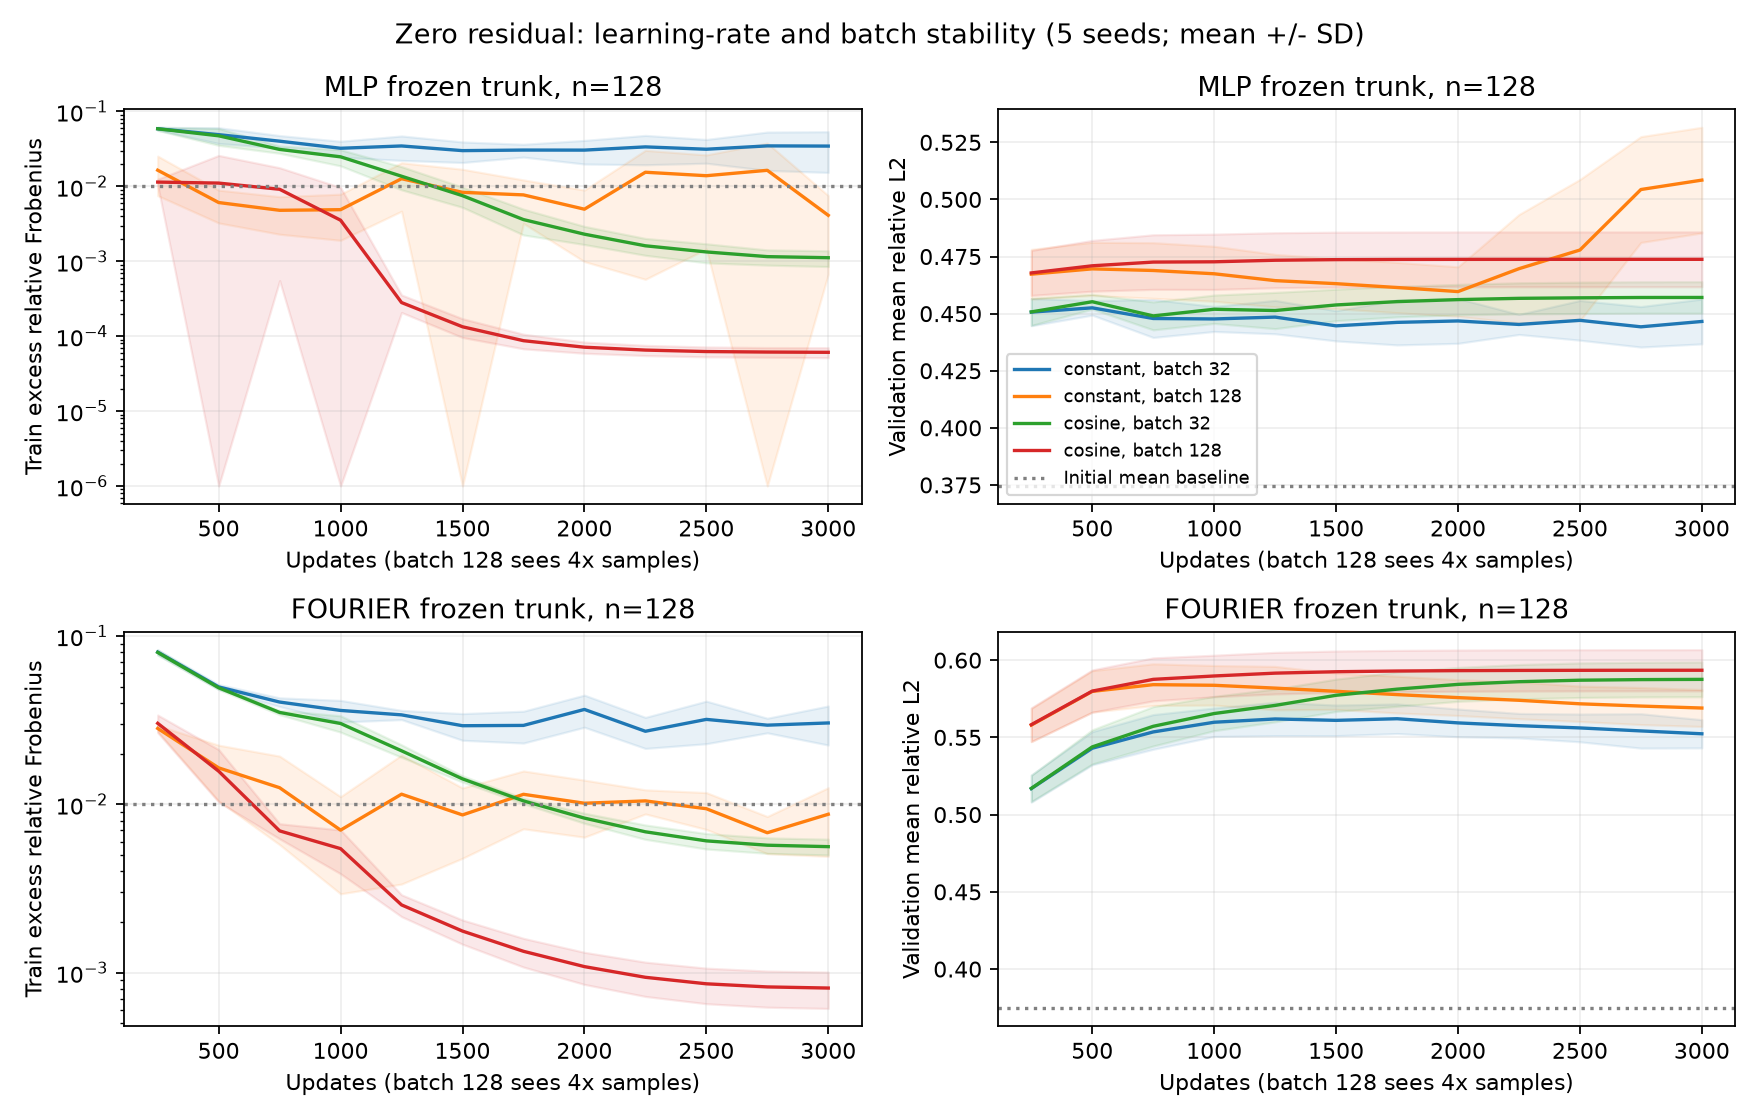
\includegraphics[width=0.85\linewidth]{stability_curves.png}
\caption{Training fit and validation behavior}
\end{figure}

Full-batch trials process four times as many examples at equal updates. Recorded update times exclude evaluation and checkpointing; equal update counts are not equal compute.

\subsection{A physics-informed arm, and where it fails}

Every result above is supervised. This arm repeats the decomposition on genuinely physics-informed training: the loss is the initial condition, the PDE residual \texttt{u\_t + u u\_x - nu u\_xx}, and periodicity, with \textbf{no supervision at the target time} (PHYSICS\_INFORMED\_V1.md). The trunk therefore takes \texttt{(t, x)} rather than \texttt{x}.

A residual can only be written once the data is known to satisfy the equation, so the coefficient was measured first (\texttt{scripts/estimate\_burgers\_nu.py}): on Nu = 0.01 the fitted convection coefficient is 0.995 and the fitted diffusion is 3.140e-3 against \texttt{nu\_file / pi} = 3.183e-3, with $R^2$ = 0.9999, whereas Nu = 0.001 fits poorly ($R^2$ = 0.79) because its shocks are under-resolved. Only Nu = 0.01 is used, with $nu = 3.083e-3$ preregistered and not tuned on any model output.

\begin{center}
\begin{adjustbox}{max width=\linewidth}
\small
\begin{tabular}{lrrrr}
\toprule
Model & relL2 & mean share & fluctuation share & \textbf{$R^2$ per sample} \\
\midrule
oracle (exact mean, zero fluctuation) & 0.32623 & 0.0000 & 0.1875 & 0.0000 \\
supervised MLP DeepONet & 0.36238 & 0.0334 & 0.1926 & -0.0273 $\pm$ 0.0159 \\
\textbf{physics-informed MLP DeepONet} & 0.43613 & \textbf{0.1246} & 0.1875 & \textbf{-0.0003 $\pm$ 0.0100} \\
supervised Fourier DeepONet & 0.38921 & 0.0510 & 0.2333 & -0.2443 $\pm$ 0.1387 \\
\textbf{physics-informed Fourier DeepONet} & 0.48460 & \textbf{0.1736} & 0.2295 & \textbf{-0.2240 $\pm$ 0.0849} \\
\bottomrule
\end{tabular}
\end{adjustbox}
\end{center}


The PDE loss fell from about 1e-1 to 6e-5, so this is a converged residual and not an unconverged run.

\textbf{Physics-informed training does not produce positive fluctuation skill}, which is what section 5.7 predicts: the residual changes what the branch is asked to fit, not its ability to represent the input-to-coefficient map. The branch-bottleneck claim survives untouched.

The decomposition says something more precise than "physics does not help". For the MLP trunk, physics-informed training reaches a fluctuation share of 0.1875 --- \textbf{exactly} the oracle's --- giving $R^2$ = -0.0003, marginally better than supervised training's -0.0273. Its total error is nevertheless much worse, and the split localises why: the \textbf{mean share rises from 0.0334 to 0.1246}. With no target-time supervision the conserved mean has to emerge from the residual and the initial condition alone, and it does not. Physics-informed training here is not worse at the fluctuation; it is worse at the conservation law.

The arm was then extended to a shorter horizon, $T = 0.5$, chosen because \textbf{supervised training succeeds there} (MLP +0.1500, Fourier +0.1878), with the prediction preregistered that physics-informed training would still fail to reach positive skill.

\begin{center}
\begin{adjustbox}{max width=\linewidth}
\small
\begin{tabular}{lrrrr}
\toprule
Model & relL2 & mean share & fluctuation share & \textbf{$R^2$ per sample} \\
\midrule
oracle (exact mean, zero fluctuation) & 0.43080 & 0.0000 & 0.2748 & 0.0000 \\
supervised MLP DeepONet & 0.41646 & 0.0169 & 0.2336 & +0.1500 $\pm$ 0.0152 \\
supervised Fourier DeepONet & 0.40288 & 0.0327 & 0.2232 & +0.1878 $\pm$ 0.0747 \\
\textbf{physics-informed MLP DeepONet} & 0.49731 & \textbf{0.0707} & 0.2724 & \textbf{+0.0088 $\pm$ 0.0054} \\
\textbf{physics-informed Fourier DeepONet} & 0.52047 & \textbf{0.1565} & 0.2606 & \textbf{+0.0516 $\pm$ 0.0364} \\
\bottomrule
\end{tabular}
\end{adjustbox}
\end{center}


\textbf{The preregistered prediction was wrong and is reported as falsified}: physics-informed training does reach positive skill at this horizon, +0.0088 and +0.0516. The loss weights and the coefficient were not adjusted in response.

What survives is the comparison and the localisation. Physics-informed skill is 17 times lower than supervised for the MLP trunk and 4 times lower for the Fourier trunk, and the \textbf{mean share is again where the damage is} (0.071 and 0.157 against 0.017 and 0.033), the same pattern as at $T = 1.0$. The corrected statement is therefore weaker and more accurate than the preregistered one: at a horizon where supervision succeeds, physics-informed training also succeeds but barely, and its deficit stays concentrated in the conserved mean rather than in the fluctuation.

A third arm uses \textbf{linear advection}, whose residual needs no fitted coefficient ($u_t + beta u_x = 0$, $beta = 0.4$ from the file attributes). It is the strongest test available because supervised skill there is high.

\begin{center}
\begin{adjustbox}{max width=\linewidth}
\small
\begin{tabular}{lrrrr}
\toprule
Model & relL2 & \textbf{$R^2$ per sample} & supervised & ratio \\
\midrule
physics-informed MLP DeepONet & 0.7115 & \textbf{-0.0033 $\pm$ 0.0044} & +0.1817 & -0.02 \\
physics-informed Fourier DeepONet & 0.5503 & \textbf{+0.3590 $\pm$ 0.0407} & +0.9424 & \textbf{0.38} \\
\bottomrule
\end{tabular}
\end{adjustbox}
\end{center}


The preregistered prediction was partially falsified again: it expected positive skill from both trunks, and the MLP trunk sits at -0.0033, indistinguishable from the zero-fluctuation reference. What survives is the ratio, and it is the more informative result. Across the three operator-horizon combinations measured, physics-informed training recovers a fraction of supervised fluctuation skill of roughly 0.06 and 0.28 on Burgers at T = 0.5, and roughly 0 and 0.38 on advection. It never approaches supervised performance; its best relative showing is on the linear operator with a Fourier trunk, consistent with translation being the easiest residual to satisfy.

\textbf{The comparison is per update, not compute-matched, and the imbalance runs against the physics-informed arm.} Measured on the same GPU from the \texttt{train\_seconds} recorded by the two training loops, one physics-informed update costs \textbf{9.4x to 12.8x} what one supervised update costs (mean 10.8x over the six operator-horizon-architecture combinations), because the residual requires second derivatives through the trunk as well as the interior collocation points. The physics-informed arm therefore received roughly an order of magnitude \emph{more} compute for the same 1500 updates and still did not reach supervised fluctuation skill. That direction favours the reported conclusion, so the correct statement is stronger than a caveat: the arm was not starved of compute, it was given more of it.

What is \emph{not} matched is the normalisation. The physics-informed arm runs a batch of 4 initial conditions against 256 collocation plus 256 initial-condition plus 64 boundary points, while the supervised arm runs a batch of 32 samples on the 256-point grid. Equal update counts therefore do not mean equal samples seen, and the two arms are not interchangeable point for point; only the decomposition quantities and their ratios should be carried across.

Further caveats: no physics-informed FNO control was run, because the 1D FNO maps a field to a field at one fixed time and has no time coordinate to differentiate; FNO appears only as the supervised reference. The arm covers two operators because only Burgers Nu = 0.01 and linear advection admit a trustworthy residual with the data available.

\subsection{A scope condition on the per-sample measures}

Every quantity above divides by each sample's own norm, so target norms spanning orders of magnitude make the per-sample numbers uninterpretable. Measured on the test split, the coefficient of variation of $||y_j||$ and the max/min spread of $||y_j||$ are:

\begin{center}
\begin{adjustbox}{max width=\linewidth}
\small
\begin{tabular}{lrr}
\toprule
family & CV & spread \\
\midrule
Burgers Nu = 0.001 & 0.65 & 59.5 \\
Burgers Nu = 0.01 & 0.66 & 90.6 \\
linear advection & 0.45 & 14.2 \\
diffusion-sorption & 0.06 & 1.3 \\
Darcy beta 1.0 / beta 10.0 & 0.54 / 0.47 & 10.7 / 7.9 \\
2D reaction-diffusion, components 0 / 1 & 0.04 / 0.07 & 1.3 / 1.6 \\
1D CFD density / Vx / pressure & 0.48 / \textbf{0.75} / 0.49 & 11.5 / \textbf{99.8} / 12.5 \\
\bottomrule
\end{tabular}
\end{adjustbox}
\end{center}


The largest values anywhere in the reported families are \textbf{CV 0.75 and a 99.8-fold spread}, both on the CFD \texttt{Vx} component. Every reported setting is therefore inside the stated scope condition below; no reported family exceeds it.

A Darcy variant at beta = 0.01 has a coefficient of variation of \textbf{2.43} and a 343-fold spread. There every architecture produced relL2 of 0.70 to 3.80 and $R^2$ of -1.9 to -87, but its validation curves are non-monotone and some seeds end worse than they started, so the run did not converge either. That setting is \textbf{excluded}: it is neither a confirmation nor a falsification of the threshold rule, and reporting it as a falsification would mistake a metric artifact plus a failed run for a measurement. The scope condition is therefore stated explicitly: the decomposition applies where target norms are of comparable scale, roughly CV below 1 and spread below 100-fold.

The same search also showed that the steady operator has \textbf{no boundary setting}: across a 1000-fold change in Darcy \texttt{beta} the target fluctuation energy only moves between 0.492 and 0.564, always far above every threshold. The threshold boundary therefore remains tested on evolution problems only.

\subsection{A system of equations, and where the rule stops holding}

The four operators above are scalar. PDEBench 1D compressible CFD supplies three coupled fields (\texttt{density}, \texttt{Vx}, \texttt{pressure}), each \texttt{(10000, 101, 1024)}, and is the first system in the study. Its protocol and six predeclared sign predictions were committed before any run (CFD\_SYSTEM\_V1.md).

The branch receives all three components at the initial time and predicts one component at $t = 1.0$; one cache is written per output component so that every downstream script applies unchanged. \textbf{FNO is not run here}: \texttt{FNO1d} requires the input and the coordinate to have equal length, which a three-channel input violates, and \texttt{src/fno.py} is hashed into every existing run identity.

The conservation structure differs \textbf{within} the system, which is measured rather than assumed: mass \texttt{mean(rho)} and momentum \texttt{mean(rho*Vx)} have input-output mean correlations of 1.000000, whereas the spatial mean of \texttt{Vx} alone does not (0.9874, a 12\% mean difference). So the input-spatial-mean predictor is a conservation-law predictor for density, approximately one for pressure, and not one for Vx --- the Darcy lesson reproduced inside a single operator.

\begin{center}
\begin{adjustbox}{max width=\linewidth}
\small
\begin{tabular}{lrrrrl}
\toprule
component & measured fluctE & MLP DeepONet & Fourier DeepONet & predicted & verdict \\
\midrule
density & 0.2651 & -0.0237 $\pm$ 0.0150 & -0.1132 $\pm$ 0.0481 & + / - & \textbf{wrong / ok} \\
Vx & 0.4659 & -0.0160 $\pm$ 0.0201 & -0.2356 $\pm$ 0.0813 & + / + & \textbf{wrong / wrong} \\
pressure & 0.0744 & -0.0448 $\pm$ 0.0759 & -0.1967 $\pm$ 0.0857 & - / - & ok / ok \\
\bottomrule
\end{tabular}
\end{adjustbox}
\end{center}


With the multi-channel FNO control added (\texttt{src/fno1d\_multi.py}), the reversal is sharper than a missing reference:

\begin{center}
\begin{adjustbox}{max width=\linewidth}
\small
\begin{tabular}{lrrrr}
\toprule
component & FNO relL2 & \textbf{FNO $R^2$ per sample} & MLP DeepONet & Fourier DeepONet \\
\midrule
density & 0.26690 & \textbf{-0.0628 $\pm$ 0.0323} & -0.0237 & -0.1132 \\
Vx & 1.12518 & \textbf{-0.8215 $\pm$ 0.4606} & -0.0160 & -0.2356 \\
pressure & 0.08858 & \textbf{-0.2501 $\pm$ 0.0689} & -0.0448 & -0.1967 \\
\bottomrule
\end{tabular}
\end{adjustbox}
\end{center}


\textbf{FNO is worse than both DeepONet trunks on \texttt{Vx} and \texttt{pressure}, and worse than the MLP trunk but not the Fourier trunk on \texttt{density} (-0.0628 +- 0.0323 against -0.1132)}, whereas on every scalar problem it is far better (+0.65 to +0.99 against -0.09 to -0.24). The FNO advantage is therefore specific to single-field inputs: it does not merely shrink on a system, it reverses. This also explains the rule's failure, since the thresholds encode a large FNO-to-DeepONet gap that exists only in the single-field case.

\textbf{Sign accuracy 3 of 6: the rule is falsified on this system for every prediction of positive skill.} The one direction that survives is the negative branch: pressure, whose fluctuation energy 0.0744 lies below every threshold, was predicted negative and is negative for both trunks. So on the system the rule retains its \emph{negative} predictive content and loses its \emph{positive} predictive content. In line with the preregistered criterion the thresholds were not refitted. The runs converged --- validation curves plateau at 0.28, 1.10 and 0.096 --- so these are measurements and not failed optimisations, unlike the excluded Darcy beta 0.01 setting.

A-priori fluctuation energy spans 0.074 to 0.542 across the three components, a range that on scalar problems straddles every threshold, and \textbf{every} measured skill is negative. The split shows pressure is predicted well in total (relL2 0.084) while its fluctuation share still exceeds the zero-fluctuation reference, so its negative $R^2$ reflects a fluctuation too small to matter rather than a poor model; Vx fails on both components of the error.

The most likely confound is the input, stated without refitting: the branch here encodes three coupled fields (768 values) rather than one (256), and the thresholds were fitted on single-field inputs. The observation is that the rule does not survive a threefold increase in input complexity. No threshold was adjusted.

\textbf{Consequence for the claims.} The threshold rule fails on this system, but section 5.14 shows it does \textbf{not} fail on systems as a class, so the failure is specific to compressible flow rather than to coupling. This is reported rather than defended.

For a multi-channel input the diagnostic's "oracle input mean" row is not interpretable --- it averages over channels whose scales differ by orders of magnitude --- so the component-wise conservation check above is the valid statement, and the skill measures, which do not use that oracle, are unaffected.

\subsection{A second system, two-dimensional: the rule recovers}

The failure above could have been a property of coupled fields in general. PDEBench 2D reaction-diffusion supplies a \textbf{second system}, and a two-dimensional one, so it separates "systems" from "compressible flow". Its protocol and four predictions were committed before any run (DIFFREACT2D\_SYSTEM\_V1.md).

As with the 1D diffusion-sorption file, two properties were measured before writing any code: the stored initial layer is broadband noise (only 4.9\% of its spectral energy inside r < 0.25 Nyquist), so it is not used, and the field smooths quickly (96.8\% of the energy is smooth by layer 20), so the input is layer 20 and the target is layer 100. This file also holds only 1000 samples, so the split is 600/200/200 rather than the 1000/200/200 used elsewhere.

\begin{center}
\begin{adjustbox}{max width=\linewidth}
\small
\begin{tabular}{lrrrl}
\toprule
component & measured fluctE & MLP DeepONet & Fourier DeepONet & predicted \\
\midrule
0 & 0.9110 & +0.0310 $\pm$ 0.0093 & +0.2377 $\pm$ 0.0060 & + / + \\
1 & 0.8282 & +0.0910 $\pm$ 0.0235 & +0.3734 $\pm$ 0.0019 & + / + \\
\bottomrule
\end{tabular}
\end{adjustbox}
\end{center}


\textbf{4 of 4: the rule holds here.}

With the multi-channel FNO control added (\texttt{src/fno2d\_multi.py}), the architecture ordering is the same as on every scalar problem:

\begin{center}
\begin{adjustbox}{max width=\linewidth}
\small
\begin{tabular}{lrrr}
\toprule
component & FNO & Fourier DeepONet & MLP DeepONet \\
\midrule
0 & \textbf{+0.9869 $\pm$ 0.0014} & +0.2377 & +0.0310 \\
1 & \textbf{+0.9879 $\pm$ 0.0053} & +0.3734 & +0.0910 \\
\bottomrule
\end{tabular}
\end{adjustbox}
\end{center}


FNO dominates here by more than 0.6 in $R^2$, exactly as it does on the scalar families, and in complete contrast to 1D compressible CFD, where FNO is the \emph{worst} of the three on \texttt{Vx} and \texttt{pressure}, though not on \texttt{density} (section 5.13). So it is not coupling, and not a multi-field input, that costs FNO its advantage; the CFD system remains the single exception in the study, on every architecture.

This corrects a narrowing that was too strong. After section 5.13 the claim had been reduced to "valid for scalar operators only"; that is wrong. The corrected statement is that the rule holds on every scalar family tested, with three held-out confirmations, \textbf{and} on 2D reaction-diffusion, and fails on 1D compressible CFD. Its failure is therefore \textbf{specific to that operator}, not a property of coupled fields.

What distinguishes the two systems is \textbf{not established} by this study. They differ in PDE type (parabolic reaction-diffusion against hyperbolic compressible flow), in fluctuation energy (0.83-0.91 against 0.07-0.47), and in the number of components, all at once. The most tempting reading is the middle row --- that the positive branch fails in a middle range of fluctuation energy and holds when it is very high --- but that is a hypothesis, not a finding. Both systems are predicted poorly in total terms (best relL2 0.66 to 1.10), so it is the fluctuation measure and not overall accuracy that separates them.

\subsection{Where the rule holds, and what the three misses share}

Across the six held-out evaluations the rule made \textbf{55 preregistered sign predictions and 52 were correct}: 18 of 18 on diffusion-sorption, 21 of 21 on Burgers at Nu = 0.01, 3 of 3 on Darcy beta 1.0, 3 of 3 on Darcy beta 10, 4 of 4 on 2D reaction-diffusion, and 3 of 6 on 1D compressible CFD. The thresholds were never refitted on any held-out family. All three misses are on that single operator, so the question is what is distinctive about it. Section 5.16 asks how much this count is worth, because the 55 are not equally informative.

Three candidate explanations can be \textbf{eliminated with the data already collected}:

\begin{center}
\begin{adjustbox}{max width=\linewidth}
\small
\begin{tabular}{ll}
\toprule
candidate & evidence that removes it \\
\midrule
coupled fields in general & 2D reaction-diffusion is a two-component system and scores 4 of 4 \\
a multi-field branch input & the same system has a two-field input and holds \\
the level of fluctuation energy & Darcy beta 1.0 at 0.4964 holds while CFD Vx at 0.4659 fails; nearly equal energies, opposite outcomes \\
\bottomrule
\end{tabular}
\end{adjustbox}
\end{center}


What the misses do share is shown below.

\begin{center}
\begin{adjustbox}{max width=\linewidth}
\small
\begin{tabular}{lrrrl}
\toprule
CFD component & $R^2$ per sample (MLP) & $R^2$ per sample (Fourier) & mean share (MLP) & spatial mean conserved? \\
\midrule
density & -0.0237 & -0.1132 & 0.011 & yes, 1.000000 \\
Vx & -0.0160 & \textbf{-0.2356} & \textbf{0.598} & \textbf{no, 12\% difference} \\
pressure & -0.0448 & -0.1967 & 0.0007 & approximately, 0.6\% \\
\bottomrule
\end{tabular}
\end{adjustbox}
\end{center}


Two of the three misses (density and Vx, MLP trunk) sit inside |$R^2$| < 0.03, a band where the measured skill is not distinguishable from the zero-fluctuation reference, so they are sign flips on an essentially flat quantity rather than substantive failures. The one miss with real magnitude is \textbf{Vx on the Fourier trunk at -0.2356}, and Vx is the only setting anywhere in this study with two properties at once: its \textbf{mean share dominates the error} (0.598 for the MLP trunk, 0.747 for Fourier), and its \textbf{spatial mean is not conserved} --- momentum is conserved but velocity is not (section 5.13).

For scale, the largest family-mean mean share anywhere outside this system is \textbf{0.051} (supervised Fourier DeepONet on Burgers at $Nu = 0.01$, section 5.11); the Burgers $Nu = 0.001$ family of section 5.2 reaches 0.034. The only other place where the mean share is comparable to CFD \texttt{Vx} is the \textbf{physics-informed arm} (0.071 and 0.157, section 5.11), and there the cause is known and different: with no supervision at the target time, the conserved mean is precisely what is not learned. On CFD \texttt{Vx} the mean share dominates under ordinary supervised training, which is what makes it the outlier.

So the failure is localised rather than explained. The rule is right on 52 of 55 held-out predictions; every miss is on one operator; two of them are marginal; and the one substantial miss is on the only component whose error is dominated by a mean the input does not determine. We do not claim a cause, and we did not adjust anything in response.

\subsection{How much the 52 of 55 is worth}

The headline count is honest but easy to over-read, because the 55 predictions are not equally informative. \texttt{experiments/prediction\_ledger.json} records every prediction with the a-priori fluctuation energy, the threshold, the predicted sign and the measured value with its seed standard deviation; \texttt{scripts/analyze\_prediction\_ledger.py} recomputes the count inside strata and against a trivial baseline. Three cuts matter.

\begin{center}
\begin{adjustbox}{max width=\linewidth}
\small
\begin{tabular}{lrrrl}
\toprule
stratum & n & correct & accuracy & 95\% Wilson CI \\
\midrule
all & 55 & 52 & 94.5\% & [85.1, 98.1] \\
saturated (measured $R^2 >= 0.9$) & 25 & 25 & 100.0\% & [86.7, 100.0] \\
informative (not saturated) & 30 & 27 & 90.0\% & [74.4, 96.5] \\
boundary (within 15\% of the threshold) & 6 & 5 & 83.3\% & [43.6, 97.0] \\
resolvable ($|R^2| > 2 sd$) & 47 & 46 & 97.9\% & [88.9, 99.6] \\
not resolvable & 8 & 6 & 75.0\% & [40.9, 92.9] \\
informative \textbf{and} resolvable & 22 & 21 & 95.5\% & [78.2, 99.2] \\
\bottomrule
\end{tabular}
\end{adjustbox}
\end{center}


(The rows above are the output of \texttt{scripts/analyze\_prediction\_ledger.py} verbatim, and \texttt{tests/test\_prediction\_ledger.py} asserts they still match, so the table cannot drift from the ledger.)

\begin{enumerate}
\item \textbf{25 of the 55 are nearly free.} On diffusion-sorption every setting scores above 0.998, and on Darcy the two non-MLP arms score above 0.91; where a model is essentially perfect the sign is not in doubt and the prediction cannot discriminate between methods. The rule is 25 of 25 there, which says little. The saturated cut is \textbf{signed on purpose}: a large negative $R^2$ is a decisive failure and stays in the informative set.
\item \textbf{Only six predictions test the rule where it could go either way} --- those whose fluctuation energy lies within 15\% of the relevant threshold. They are the two Burgers $Nu = 0.01$ trunks at $t = 0.75$ (whose energies straddle the two thresholds and for which the rule therefore makes \emph{opposite} predictions on the same target), MLP at $t = 1.00$, FNO at $t = 1.50$, and both CFD density trunks. The rule is \textbf{5 of 6} there, and the single miss is CFD density on the MLP trunk, at \texttt{-0.0237 $\pm$ 0.0150}.
\item \textbf{Eight predictions are not statistically resolvable} --- the measured value is within two seed standard deviations of zero, so their sign is partly a coin flip. The rule is 6 of 8 there and 46 of 47 where the sign \emph{is} resolvable. Two of the three misses are non-resolvable; the one miss with real magnitude is CFD \texttt{Vx} on the Fourier trunk at \texttt{-0.2356 $\pm$ 0.0813} (2.9 sd).
\end{enumerate}


\textbf{Baseline.} The rule predicted \texttt{+} in 44 of 55 cases, so the obvious skeptical baseline is "always predict positive". That baseline scores 41 of 55 (74.5\%, CI [61.7, 84.2]) overall but only \textbf{16 of 30 (53.3\%, CI [36.1, 69.8])} on the informative subset, against the rule's 27 of 30 (90.0\%, CI [74.4, 96.5]). The two intervals do not overlap on the informative subset, which is the comparison that matters: on the easy saturated settings the baseline does nearly as well, and it is the discriminating settings that separate the rule from it.

We therefore state the result as \textbf{27 of 30 on informative predictions, 5 of 6 at the threshold boundary}, and report 52 of 55 only as the raw count. The ledger is machine-readable and the strata are recomputed by test rather than transcribed.

\subsection{Replication on a disjoint split}

Every number above comes from one split whose test set was seen during exploratory development. Section 5.15 preregisters the \emph{rule} against later families, which protects it from hindsight but not the split from it. We therefore replicated the study on a second split, under the protocol committed in docs/REPLICATION\_SPLIT2\_V1.md before any run on it.

Split 2 uses seed 20261028 and is drawn from the \textbf{complement} of all 1400 split-1 ids, so the two splits share no trajectory. This matters: two bare seeds over 10000 trajectories would be expected to overlap on about 196 samples, which is not an independent sample. The thresholds were \textbf{refitted on split 2} rather than carried over, so what is replicated is the procedure rather than the number. All 21 families were retrained (315 runs) and every diagnostic recomputation reproduces its stored metric exactly.

\textbf{Primary endpoint: the dissociation replicates.} Burgers Nu = 0.001 at $t = 1.00$, test split:

\begin{center}
\begin{adjustbox}{max width=\linewidth}
\small
\begin{tabular}{lrr}
\toprule
 & split 1 & split 2 \\
\midrule
MLP DeepONet per-sample $R^2$ & -0.0042 $\pm$ 0.0072 & \textbf{-0.0003 $\pm$ 0.0167} \\
FNO per-sample $R^2$ & +0.6503 $\pm$ 0.0222 & \textbf{+0.6162 $\pm$ 0.0347} \\
FNO - MLP gap & +0.6545 & \textbf{+0.6165} \\
\bottomrule
\end{tabular}
\end{adjustbox}
\end{center}


All three fall inside the predeclared bands, so R0 passes. \textbf{The dissociation is not an artifact of one split.}

\textbf{Secondary endpoint: thresholds are stable where they exist.} MLP moved 0.2477 $\to$ \textbf{0.2444} (1.3\% drift) and Fourier 0.2728 $\to$ \textbf{0.3045} (11.6\% drift), both inside the 25\% band with the ordering preserved. \textbf{The FNO branch has no threshold on split 2 at all}: FNO's measured per-sample fluctuation $R^2$ stays positive across all seven fitting horizons, reaching +0.0972 $\pm$ 0.1689 at $t = 2.00$ where split 1 gave -0.0586 $\pm$ 0.2357. With no sign change there is nothing to interpolate, so the rule issues no FNO prediction. That is not a miss --- nothing was predicted and nothing was wrong --- but it removes the FNO arm from the replication, and it shows that section 5.5's statement that FNO falls below zero at $t = 2.00$ is split-dependent. On split 2 it does not cross, though at +0.0972 $\pm$ 0.1689 the margin is not distinguishable from zero either way.

\textbf{Secondary endpoint: held-out signs, 13 of 14.} With FNO unscored, the 21 preregistered predictions become 14 (two architectures, seven horizons).

\begin{center}
\begin{adjustbox}{max width=\linewidth}
\small
\begin{tabular}{rrllrl}
\toprule
t & fluctE & architecture & predicted & measured &  \\
\midrule
0.10 & 0.5721 & MLP & + & \textbf{+0.1798 $\pm$ 0.0119} & correct \\
0.10 & 0.5721 & Fourier & + & \textbf{+0.6467 $\pm$ 0.0271} & correct \\
0.25 & 0.4551 & MLP & + & \textbf{+0.1409 $\pm$ 0.0163} & correct \\
0.25 & 0.4551 & Fourier & + & \textbf{+0.3680 $\pm$ 0.0220} & correct \\
0.50 & 0.3403 & MLP & + & \textbf{+0.0555 $\pm$ 0.0434} & correct \\
0.50 & 0.3403 & Fourier & + & \textbf{+0.0318 $\pm$ 0.1243} & correct \\
0.75 & 0.2678 & MLP & + & \textbf{-0.0332 $\pm$ 0.0708} & \textbf{wrong} \\
0.75 & 0.2678 & Fourier & - & \textbf{-0.4405 $\pm$ 0.3456} & correct \\
1.00 & 0.2190 & MLP & - & \textbf{-0.1032 $\pm$ 0.1055} & correct \\
1.00 & 0.2190 & Fourier & - & \textbf{-0.8114 $\pm$ 0.2929} & correct \\
1.50 & 0.1597 & MLP & - & \textbf{-0.1206 $\pm$ 0.0334} & correct \\
1.50 & 0.1597 & Fourier & - & \textbf{-0.8781 $\pm$ 0.0611} & correct \\
2.00 & 0.1248 & MLP & - & \textbf{-0.0431 $\pm$ 0.0453} & correct \\
2.00 & 0.1248 & Fourier & - & \textbf{-0.5368 $\pm$ 0.1474} & correct \\
\bottomrule
\end{tabular}
\end{adjustbox}
\end{center}


\textbf{13 of 14} (92.9\%, CI [68.5, 98.7]) against \textbf{6 of 14 (42.9\%, CI [21.4, 67.4])} for always predicting positive. The two splits agree on where the rule is fragile: the only miss on split 2 is Burgers Nu = 0.01 at $t = 0.75$ on the MLP trunk, measured at -0.0332 $\pm$ 0.0708, i.e. within two seed standard deviations of zero --- the same statistically unresolvable band that produced two of split 1's three misses.

\textbf{What this settles and what it does not.} The dissociation, the horizon decay and the approximate threshold values are reproducible on trajectories none of which entered split 1. It does \textbf{not} close the gap identified above: the held-out family is still Burgers at a second viscosity, so the replication demonstrates stability across \emph{data}, not reach across \emph{operator classes}. It also produced one observation the single-split study could not have made --- that the FNO branch of the rule is not re-fittable on this split --- which is recorded in section 9 of the protocol. Artifacts: \texttt{results/rs2\_fluctuation/**}, \texttt{experiments/prediction\_ledger\_rs2.json}, \texttt{results/rs2\_skill\_prediction\_v1/report.json}, \texttt{results/rs2\_*/}.

\subsection{Zero initialization helps, but fitting and generalization remain distinct}

Zero initialization improves final validation relative L2 in 29/30 paired comparisons; all six group means and seed standard deviations improve. The exception is Fourier at n=1000, seed 2. Shared inputs and related seeds do not constitute 30 independent datasets, so no aggregate significance claim is made. The best zero-init validation group, MLP/n=1000 at 0.38981, still trails the validation conservation-law baseline of 0.374509.

\subsection{Practical guidance: what to report}

A diagnostic earns its keep only if it changes what gets written down. For a learned surrogate of a PDE with a conserved spatial mean, three numbers are cheap and each answers a different question.

\begin{enumerate}
\item \textbf{Report the mean share, not only total relative L2.} If the mean share is near 1, the model is level with the conservation law and predicting nothing beyond it. Total relative L2 cannot separate these cases, because the conserved mean is the easy part and it sits in the denominator.
\item \textbf{Report per-sample fluctuation $R^2$ alongside the energy-weighted one.} The two disagree in sign on Burgers $Nu = 0.001$ (section 5.4), and which is chosen determines whether the same result reads as success or failure. Say which is the headline.
\item \textbf{State the forecast horizon and re-measure at it.} Trunk quality is horizon-dependent: the Fourier trunk leads the MLP trunk by +0.2553 at $t = 0.25$ and trails it by -0.0892 at $t = 1.00$ (section 5.5). A claim about basis quality that omits the horizon is incomplete.
\end{enumerate}


Two warnings follow. Optimising total relative L2 can make the per-sample fluctuation measure \textbf{worse} (section 5.10), so total error is not a safe proxy for fluctuation skill. And a per-sample $R^2$ within two seed standard deviations of zero is not evidence of skill in either direction: report the interval, not the sign of the point estimate.

\section{Interpretation and limitations}

The supported finding is a \textbf{localization}: on this protocol the error of both DeepONet variants is dominated by a component they do not predict at all, and the component is identified as the deviation from the conserved spatial mean. FNO predicts it.

The second finding is that this is a matter of degree, not kind. On Burgers every architecture loses its fluctuation skill as the forecast horizon grows, including FNO, so the primary variable is task difficulty and the architecture sets where the boundary lies. The skill horizon quantifies that boundary and is the most directly reusable number in this study: it converts "DeepONet is worse here" into "at this viscosity and grid, MLP DeepONet stops predicting the fluctuation at t about 0.98, FNO at about 1.94".

The third finding is what the second PDE provides. On linear advection the fluctuation energy is horizon-independent and no architecture develops a skill horizon at all, so the decay is not a generic cost of forecasting further ahead: it tracks nonlinear spectral evolution and disappears when that evolution is absent.

We do \textbf{not} claim that DeepONet cannot learn fluctuations in general: at t=0.10 it scores +0.22 to +0.64. We do not claim a causal mechanism, and we do not claim FNO is universally superior; at t=2.00 FNO is below zero as well.

Limitations:

\begin{itemize}
\item Six operator families, eight setting-instances: linear transport; nonlinear convection-diffusion at two viscosities; dissipative parabolic; one steady elliptic two-dimensional problem at two \texttt{beta} values; a three-field compressible system; and a two-field two-dimensional reaction-diffusion system. Most families are studied at one parameter setting each. Splits are 1000/200/200 except the reaction-diffusion file, which holds only 1000 samples and uses 600/200/200. No shallow-water data exists in the deposit used.
\item \textbf{Benchmark age and data version.} The PDEBench \emph{paper} is 2022 [4], but the \emph{data} is a separately versioned deposit: we use DaRUS \texttt{doi:10.18419/darus-2986} \textbf{version 8, released 2024-02-13, the latest released version as of 2026-10-08}. The files were downloaded between 2026-09-22 and 2026-10-08, so they are the current upstream content rather than an archived 2022 snapshot. Maintenance of the \emph{code} repository is a separate matter and does not by itself change any data byte: the Burgers file is fetched from the HuggingFace \texttt{pdebench/Burgers} dataset pinned to git revision \texttt{97bf5bb5315b9a083b4f9fc03e5c84d35286d52c}, and the other seven files from DaRUS. Every file is byte-pinned (section 4), so the results are reproducible on the exact bytes used regardless of any future upstream revision. PDEBench remains the most widely used public benchmark for time-dependent operator learning with ground-truth trajectories, but newer surrogate-benchmark frameworks exist (for example PDEArena). Because our claim is a \emph{diagnostic decomposition} and not a state-of-the-art accuracy result, the conclusion does not depend on the benchmark being current; a reader should nevertheless read the absolute error levels as 2024-generation baselines rather than as a comparison against the newest architectures. Nothing here is claimed to transfer to foundation-model-scale operator training. A version history of the deposit is kept outside the manuscript in docs/PDEBENCH\_DATA\_VERSIONS\_V1.md.
\item \textbf{The threshold rule holds on every scalar family tested and on 2D reaction-diffusion, and fails on 1D compressible CFD} (sections 5.13 and 5.14), with the thresholds unrefitted throughout. Why CFD fails is not established, and any use of the rule on a compressible hyperbolic system is unsupported by this study.
\item Two families are weak in the specific sense that every model saturates far from the thresholds: diffusion-sorption, whose target fluctuation lies in one spatial mode and whose stored initial state is spatially constant (so it is used from layer 20 onward), and Darcy, whose only setting is far above every threshold. The quantitative boundary evidence rests on the viscosity ladder alone.
\item \textbf{Compute is measured and matched, but the match rests partly on an estimate.} Parameter counts are within 18\% and FNO costs about 2.2x more wall-clock per update, so the gap is not explained by DeepONet having less of either. A FLOP-matched control was run at the measured dense FLOP budget (5135 and 4233 updates) and again at a budget that adds an analytic FFT term (6744 and 5559 updates); the gap survives both and is larger at the larger budget, and DeepONet given 3.9x the FLOP budget is still negative (section 5.9). The remaining limitation is that the FFT portion of the FNO count is an analytic estimate rather than a measurement, because \texttt{torch.utils.flop\_counter} registers no FFT op. The estimated part belongs to FNO, so the direction of any error in it favours FNO, but equal \emph{estimated} FLOPs are still not provably equal real work.
\item \textbf{Split 1 is still the reference for section 5.15, but the study is no longer single-split.} The test split was exposed during exploratory development and validation guided later study choices, so the numbers in sections 5.2-5.16 are descriptive. The dissociation, the horizon decay and the threshold values were then \textbf{replicated on a second split sharing no trajectory with the first}, with the thresholds refitted on it, under the protocol predeclared in docs/REPLICATION\_SPLIT2\_V1.md and committed before any run (section 5.17). Two limitations survive that replication unchanged: the held-out family is still Burgers at a second viscosity rather than a new operator class, and the five seeds still share one split.
\item Five seeds share one data split, so seed standard deviations do not measure task variability.
\item Numerical-rank sensitivity of the projection oracle (rcond 1e-12 versus 1e-6) is reported in the retained diagnostic section and affects how basis quality is read.
\end{itemize}


\section{Historical correctness audit and withdrawn claims}

The project previously found shared-grid helpers called on per-sample coordinates, producing \texttt{(B,B,N)} instead of \texttt{(B,N)}. Current sampler tests compare batched evaluation against an independent per-sample oracle. This is an implementation lesson, not evidence that other published systems contain the same bug.

We withdraw the old residual assertion as a mathematical test: small value error does not ensure small derivative error or PDE residual. Earlier claims that test relative L2 minus a truncated captured-energy proxy is pure optimization error, that alignment has a problem-independent variance floor, that output-NTK/sharpness correlations establish a causal mechanism, and that a modal shrinkage rule beats strong controls are not maintained. The modal-shrinkage line failed its predeclared confirmation (0 of 12 comparisons against strong controls) and is closed. Historical unknown source fingerprints remain unknown; historical p-values are not reused as confirmatory evidence. Full records remain archived, and the endpoint of a failed study was not replaced by a secondary metric.

\section{Reproducibility and next confirmation}

Versioned result directories contain manifests, events, final metrics and summaries. Dataset SHA-256, exact row identities, code hashes and environment records are retained. Large downloaded data and resumable checkpoints remain local rather than in Git; the data is not redistributable in any case, since the PDEBench deposit exceeds 50 GB. The \textbf{code} is released as a versioned archive with a DOI (see the Data availability statement before the references), which is what makes the pinned bytes retrievable: the repository records the download scripts and the byte-level digests, so the release is a carrier for the code rather than for the data.

Recomputation is enforced rather than assumed: \texttt{scripts/diagnose\_fluctuation.py} refuses to proceed if the pair cache hash changed, and reports any run whose recomputed metric differs from its stored value beyond a tolerance. The test suite asserts the exact squared-error closure, the invariance of the skill measure to the mean, and that stored metrics are reproduced.

Next experiments, in priority order: (i) \emph{completed} --- the disjoint-split replication of docs/REPLICATION\_SPLIT2\_V1.md ran in full (315 runs, 21 families) with the thresholds refitted on split 2; see section 5.17 and section 9 of the protocol for the outcomes, including the FNO arm dropping out; (ii) a FLOP counter that registers FFT work, so that the matched comparison in section 5.9 rests on a measurement rather than on the analytic estimate it currently uses; (iii) \emph{partly completed} --- the work-per-update imbalance between the physics-informed arm of section 5.11 and the supervised runs is now measured (roughly 10x, in favour of the physics-informed arm) but still not matched, and the physics-informed FNO control remains unavailable because the present 1D FNO maps a field to a field at one fixed time and has no time coordinate to differentiate; (iv) a compressible system at a second parameter set, which is what would separate the three candidate explanations that section 5.15 leaves open for the 1D CFD failure, and whose minimum available size (about 55 GB) is the reason it has not been run. No shallow-water or incompressible multi-dimensional system exists in the deposit used, so that class remains untested.





\section*{Declaration of competing interest}

The author declares that he has no known competing financial interests or personal relationships that could have appeared to influence the work reported in this paper.

\section*{Funding}

This research received no funding from any public, commercial or not-for-profit body. No employer resources were used.

\section*{Data availability}

The datasets are not redistributed with this paper: the PDEBench deposit exceeds 50 GB and is obtained from the publishers cited in section 4. Every input file is byte-pinned by SHA-256 or MD5 together with a publisher revision identifier (\texttt{HuggingFace pdebench/Burgers} git revision \texttt{97bf5bb5315b9a083b4f9fc03e5c84d35286d52c}; DaRUS \texttt{doi:10.18419/darus-2986} version 8), and the repository provides the download scripts, so every result in this paper is reproducible on the exact bytes used. All recomputed quantities and every protocol document are retained in the repository. The code is archived with a DOI: \url{https://doi.org/10.5281/zenodo.23765688.}

\section*{Author contribution}

Single author: problem statement, decomposition and proofs, software, experiments, analysis and writing.

\section*{Relation to the author's prior thesis}

Part of this work grew out of the author's undergraduate thesis, \emph{Research and Implementation of DeepONet-Based Methods for Solving Partial Differential Equations} (Harbin Institute of Technology, May 2025), which studied a physics-informed DeepONet on a self-generated one-dimensional diffusion-reaction problem and reported that adding a residual loss improved the \textbf{total} relative L2 error to 4.80e-3.

The present paper is not a republication of that thesis. The two share only the broad topic (operator learning for PDEs) and standard background. They differ in every respect that carries evidence:

\begin{center}
\begin{adjustbox}{max width=\linewidth}
\small
\begin{tabular}{lll}
\toprule
 & prior thesis & present paper \\
\midrule
data & self-generated finite-difference solutions & PDEBench deposits, byte-pinned, downloaded 2026-09/10 \\
PDEs & one-dimensional diffusion-reaction & Burgers (two viscosities), linear advection, diffusion-sorption, Darcy, compressible CFD, reaction-diffusion \\
reported measure & total relative L2 only & exact mean/fluctuation split with Propositions 1 and 2 \\
headline claim & physics-informed training \textbf{improves} accuracy & the deficit is localised in the conserved mean; at most 0.38 of supervised fluctuation skill is recovered \\
\bottomrule
\end{tabular}
\end{adjustbox}
\end{center}


The concepts central to this paper --- the spatial-mean/fluctuation decomposition, the conserved-mean reference, the trunk-span bound, the skill horizon and the fluctuation-energy threshold --- do not appear in the thesis. No figure, table, experiment or numerical result is reproduced from it. The current paper reaches conclusions that qualify the thesis's positive claim rather than repeat it.

\section*{Acknowledgments}

The author thanks the maintainers of the PDEBench deposit for making the data publicly available under stable versioning. No named individual contributed to, reviewed or endorsed this manuscript, and the author takes sole responsibility for its contents.

\begin{thebibliography}{14}
\bibitem{}
Sanghyun Lee and Yeonjong Shin. \emph{On the training and generalization of deep operator networks}. SIAM Journal on Scientific Computing, 2024. \url{https://doi.org/10.1137/23M1598751} ; \url{https://arxiv.org/abs/2309.01020}

\bibitem{}
Emily Williams, Amanda Howard, Brek Meuris and Panos Stinis. \emph{What do physics-informed DeepONets learn? Understanding and improving training for scientific computing applications}. Journal of Computational Physics, 2026. \url{https://doi.org/10.1016/j.jcp.2026.114851} ; \url{https://arxiv.org/abs/2411.18459}

\bibitem{}
Lu Lu, Xuhui Meng, Shengze Cai, Zhiping Mao, Somdatta Goswami, Zhongqiang Zhang and George Em Karniadakis. \emph{A comprehensive and fair comparison of two neural operators (with practical extensions) based on FAIR data}. Computer Methods in Applied Mechanics and Engineering 393, 114778, 2022. \url{https://doi.org/10.1016/j.cma.2022.114778} ; \url{https://arxiv.org/abs/2111.05512}

\bibitem{}
Makoto Takamoto, Timothy Praditia, Raphael Leiteritz, Daniel MacKinlay, Francesco Alesiani, Dirk Pfl\"uger and Mathias Niepert. \emph{PDEBench: An Extensive Benchmark for Scientific Machine Learning}. NeurIPS Datasets and Benchmarks, 2022. \url{https://arxiv.org/abs/2210.07182} Data deposit: DaRUS (University of Stuttgart), \url{https://doi.org/10.18419/darus-2986} . *\emph{The paper is 2022 but the data deposit is versioned separately: this study uses version 8, RELEASED, with release and last-update timestamps of 2024-02-13}* (the latest released version, queried 2026-10-08 through the Dataverse API). All datafile identifiers used here are present in that version, and every file is byte-pinned. See section 6, "Benchmark age and data version".

\bibitem{}
Thomas Bachlechner, Bodhisattwa Prasad Majumder, Huanru Henry Mao, Garrison W. Cottrell and Julian McAuley. \emph{ReZero is all you need: fast convergence at large depth}. UAI / PMLR 161, 2021. \url{https://proceedings.mlr.press/v161/bachlechner21a.html} ; \url{https://arxiv.org/abs/2003.04887}

\bibitem{}
Ilya Loshchilov and Frank Hutter. \emph{SGDR: Stochastic Gradient Descent with Warm Restarts}. ICLR 2017. \url{https://arxiv.org/abs/1608.03983}

\bibitem{}
Nitish Shirish Keskar et al. \emph{On Large-Batch Training for Deep Learning: Generalization Gap and Sharp Minima}. ICLR 2017. \url{https://arxiv.org/abs/1609.04836}

\bibitem{}
Nicola Demo, Marco Tezzele and Gianluigi Rozza. \emph{A DeepONet multi-fidelity approach for residual learning in reduced order modeling}. Advanced Modeling and Simulation in Engineering Sciences, 2023. \url{https://doi.org/10.1186/s40323-023-00249-9} ; \url{https://arxiv.org/abs/2302.12682} (corrected 2026-10-08: the first author is Nicola Demo, not Niccolo Demo)

\bibitem{}
Koike et al. \emph{Sparse POD Mode Selection and Manifold Dimensionality Reduction with Neural Networks} (SparseModesNet). 2026. \url{https://arxiv.org/abs/2605.27756}

\bibitem{}
Lu Lu, Pengzhan Jin, Guofei Pang, Zhongqiang Zhang and George Em Karniadakis. \emph{Learning nonlinear operators via DeepONet based on the universal approximation theorem of operators}. Nature Machine Intelligence 3, 218-229, 2021. \url{https://doi.org/10.1038/s42256-021-00302-5} ; \url{https://arxiv.org/abs/1910.03193}

\bibitem{}
Zongyi Li, Nikola Kovachki, Kamyar Azizzadenesheli, Burigede Liu, Kaushik Bhattacharya, Andrew Stuart and Anima Anandkumar. \emph{Fourier Neural Operator for Parametric Partial Differential Equations}. ICLR 2021. \url{https://arxiv.org/abs/2010.08895}

\bibitem{}
Siavash Khodakarami, Vivek Oommen, Nazanin Ahmadi Daryakenari et al. \emph{Spectral bias in physics-informed and operator learning: Analysis and mitigation guidelines}. Computer Methods in Applied Mechanics and Engineering, 2026. \url{https://www.sciencedirect.com/science/article/pii/S0045782526004299} ; \url{https://arxiv.org/abs/2602.19265}

\bibitem{}
Mark Ainsworth and J. Tinsley Oden. \emph{A Posteriori Error Estimation in Finite Element Analysis}. Wiley-Interscience, 2000.

\bibitem{}
Roland Becker and Rolf Rannacher. \emph{An optimal control approach to a posteriori error estimation in finite element methods}. Acta Numerica 10, 1-102, 2001. \url{https://doi.org/10.1017/S0962492901000010}

\end{thebibliography}

\end{document}
